\graphicspath{{Ch6_Results/figures/}}

\chapter{Results}
\label{ch:results}
In this section the results of the combined fit with the full 2015, 2016, 2017, and 2018 datasets will be presented, corresponding to a total integrated luminosity of \lumi.

\section{Post-Fit Dijet Mass}

Post-fit studies performed on various mass points for both WH and ZH final states are used to verify the integrity of the fits.
In all cases, stable results are obtained and only a representative set of studies is shown in this section.
Figure~\ref{fig:post_fit_2p6TeV} shows the resulting post-fit \mvh\ distributions.
The pulls and constraints on the nuisance parameters are shown in Figure ~\ref{fig:pull_plots} for the WH 2.6 TeV and ZH 4.0 TeV mass points.
The ranking of nuisance parameters are shown in Figures~\ref{fig:rank_plots_2p6TeV} and~\ref{fig:rank_plots_4TeV} for 2.6 TeV and 4.0 TeV signal mass points, respectively.

%TODO: In figure captions better explain ranking plot, correlation matrix, etc
\begin{figure}[htbp!]
    \begin{center}
        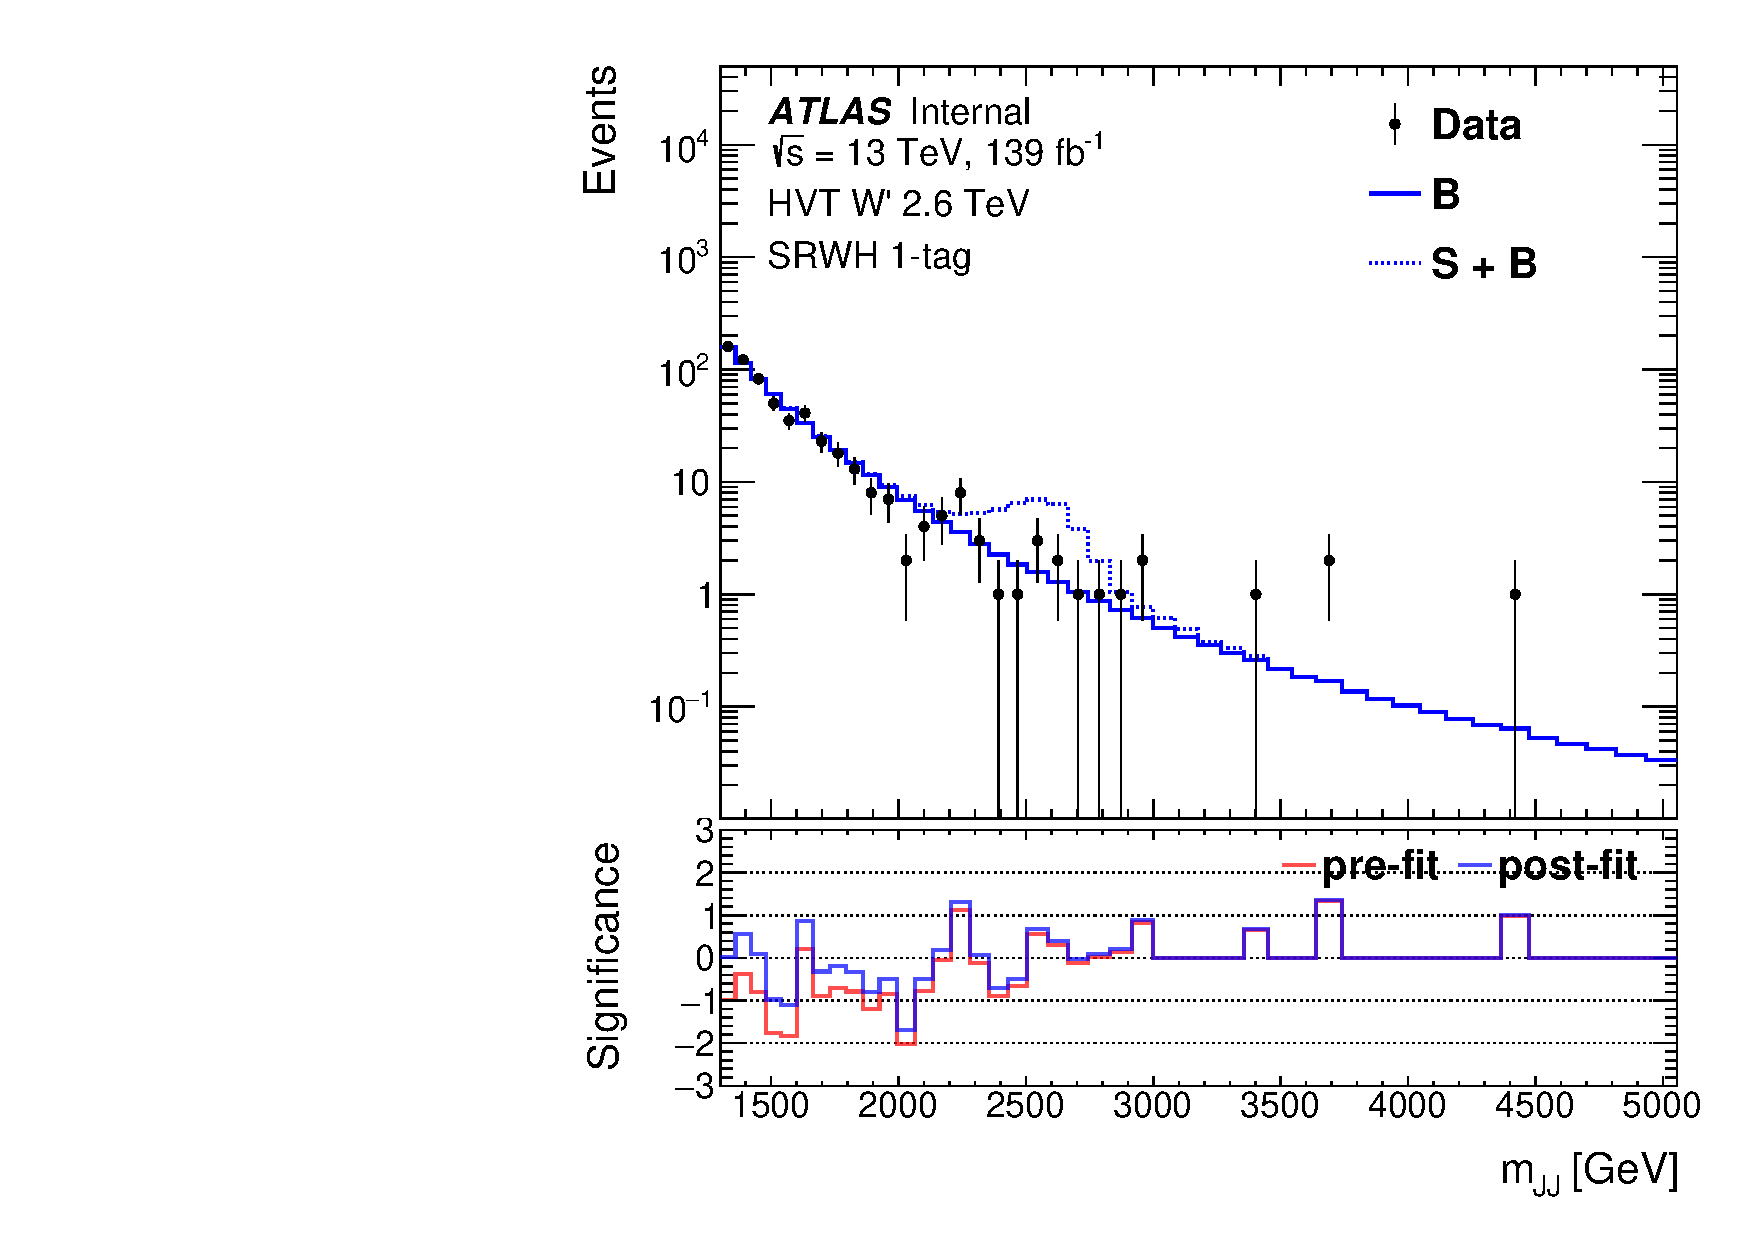
\includegraphics[width=0.49\textwidth]{VHqqbbPrePostFit_Chqqbb_SRWH_1tag_mVH_2600.pdf}
        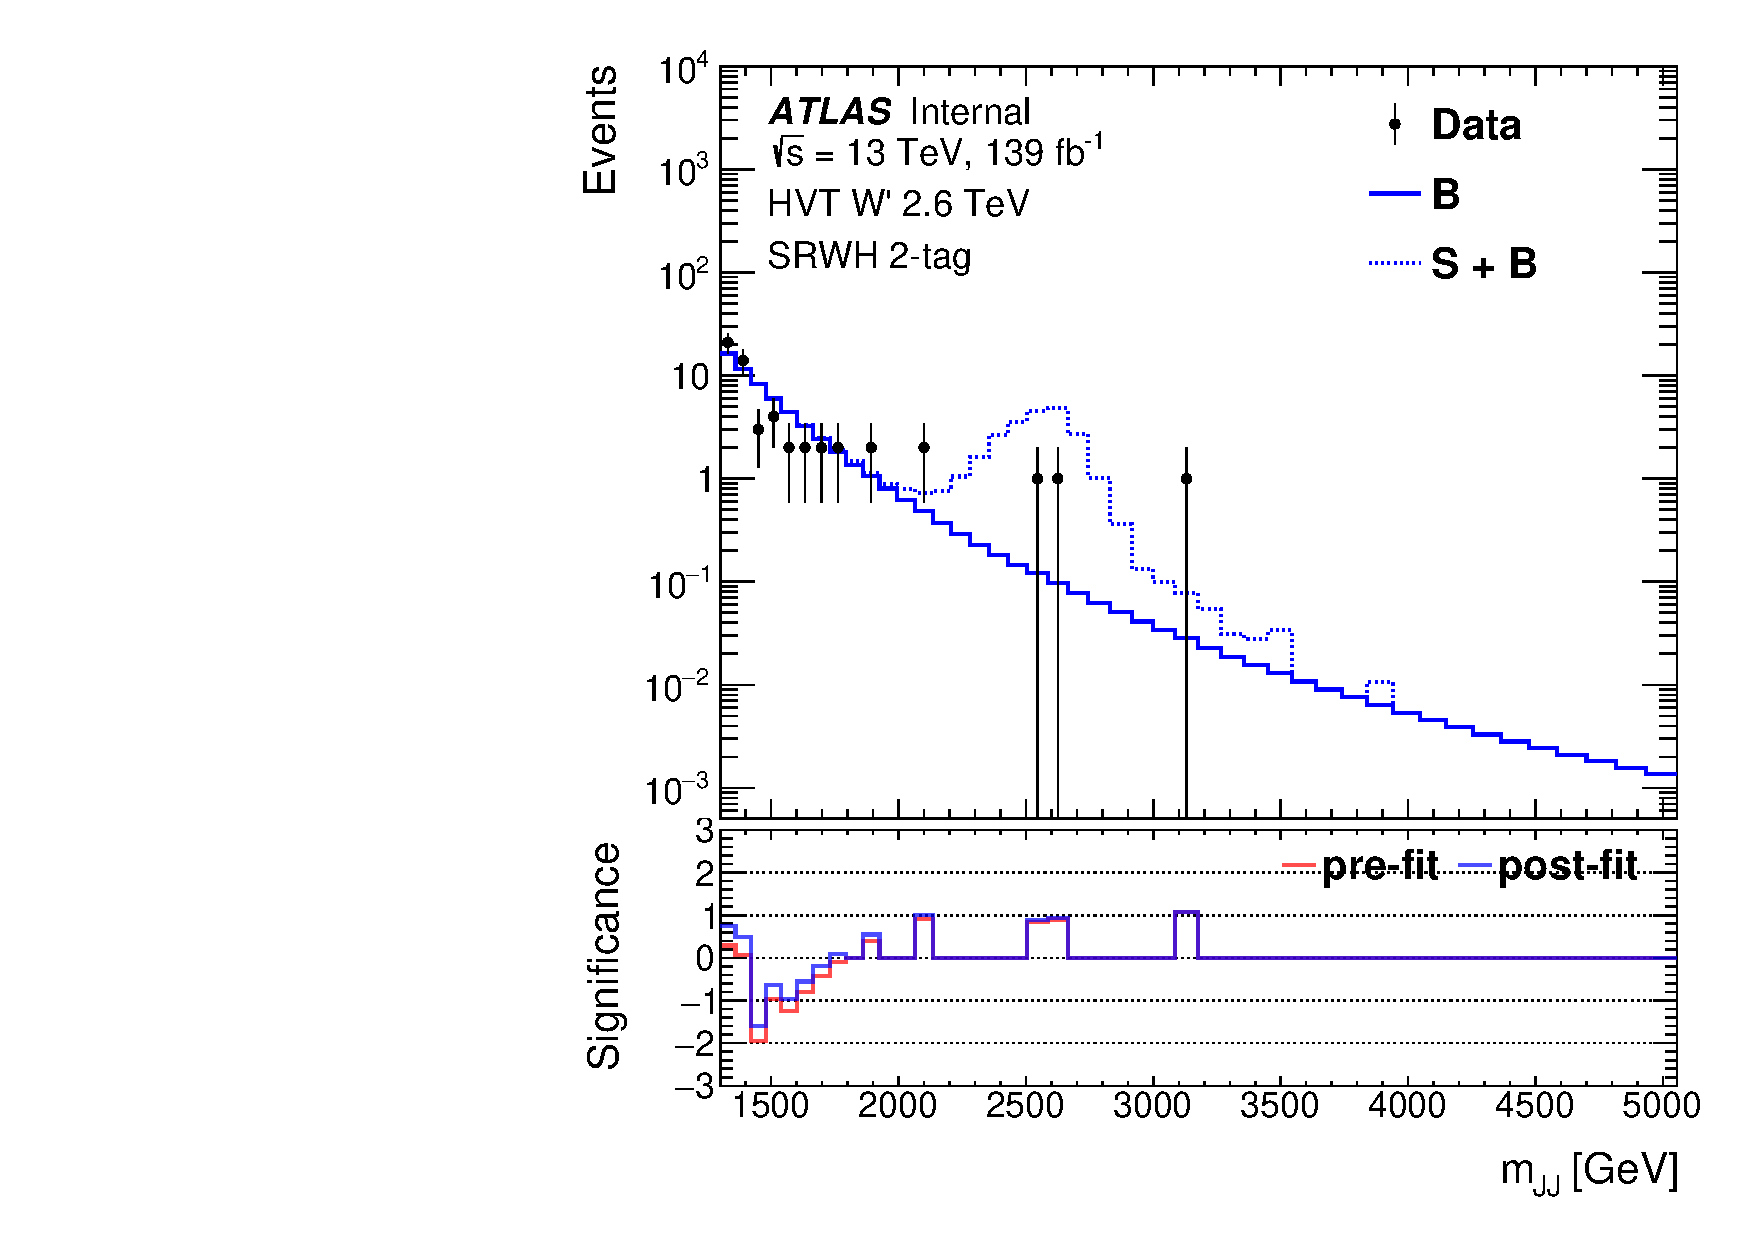
\includegraphics[width=0.49\textwidth]{VHqqbbPrePostFit_Chqqbb_SRWH_2tag_mVH_2600.pdf} \\
        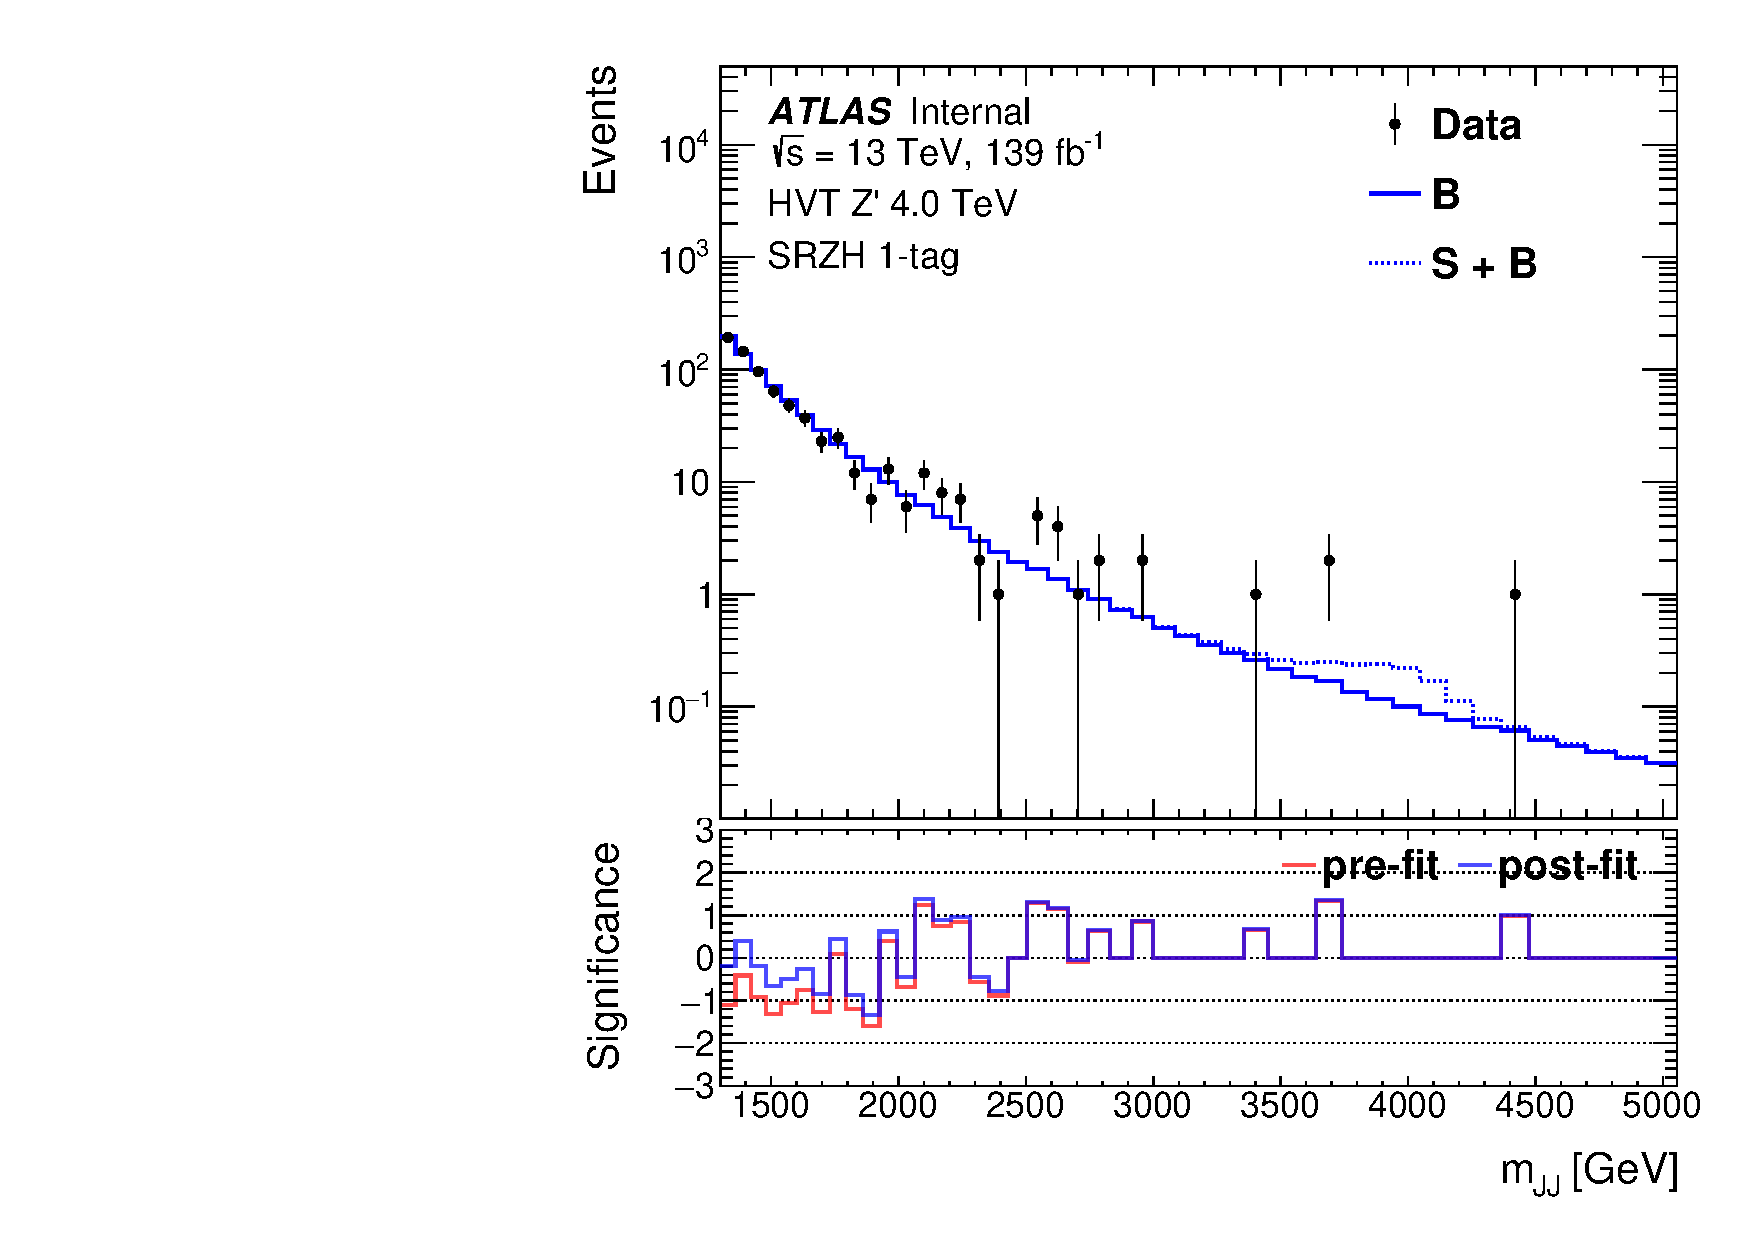
\includegraphics[width=0.49\textwidth]{VHqqbbPrePostFit_Chqqbb_SRZH_1tag_mVH_4000.pdf}
        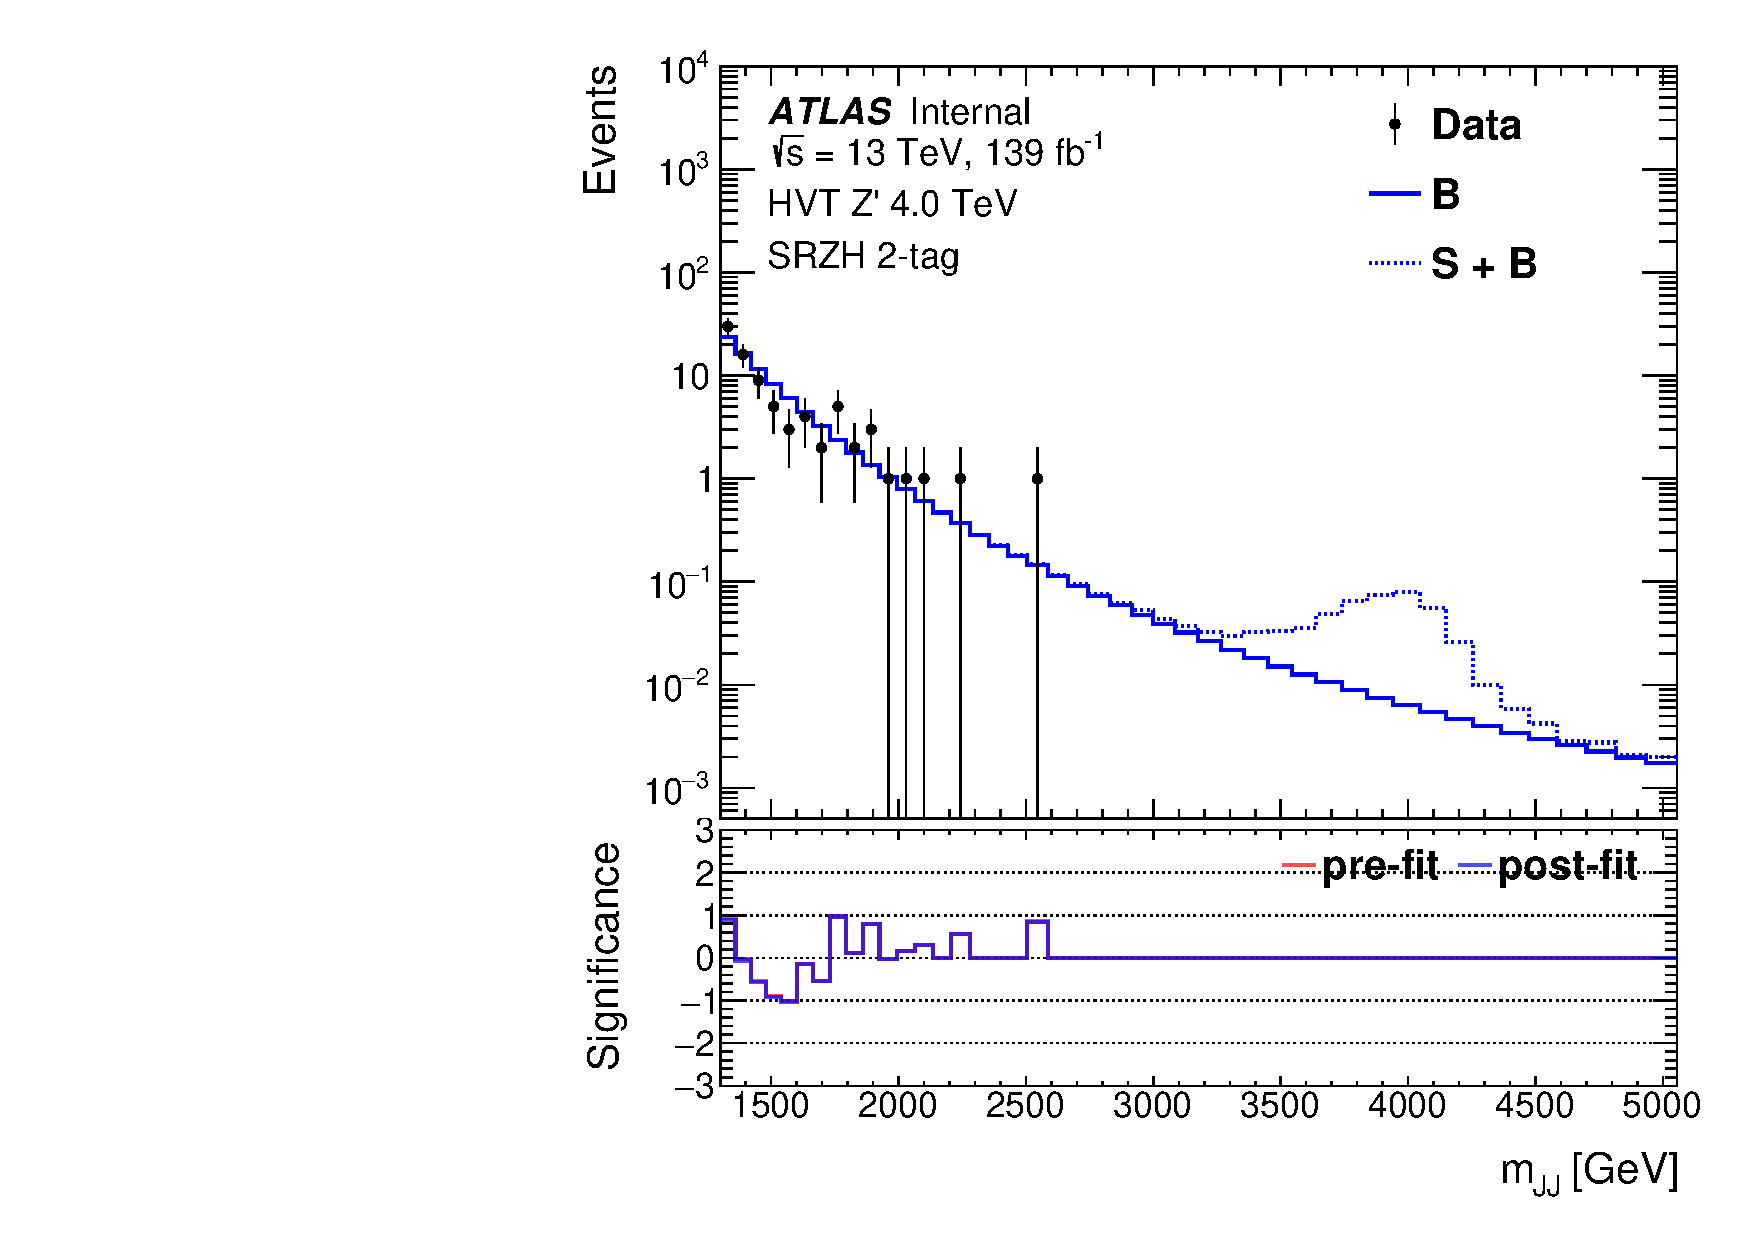
\includegraphics[width=0.49\textwidth]{VHqqbbPrePostFit_Chqqbb_SRZH_2tag_mVH_4000.pdf}
    \end{center}
    \caption{Post-fit \mvh\ distribution for the 2.6 TeV mass point in SRWH (top row) and SRZH (bottom row) for both the 1-tag (left) and 2-tag (right) channels.}
    \label{fig:post_fit_2p6TeV}
\end{figure}

\begin{figure}[htbp!]
    \begin{center}
        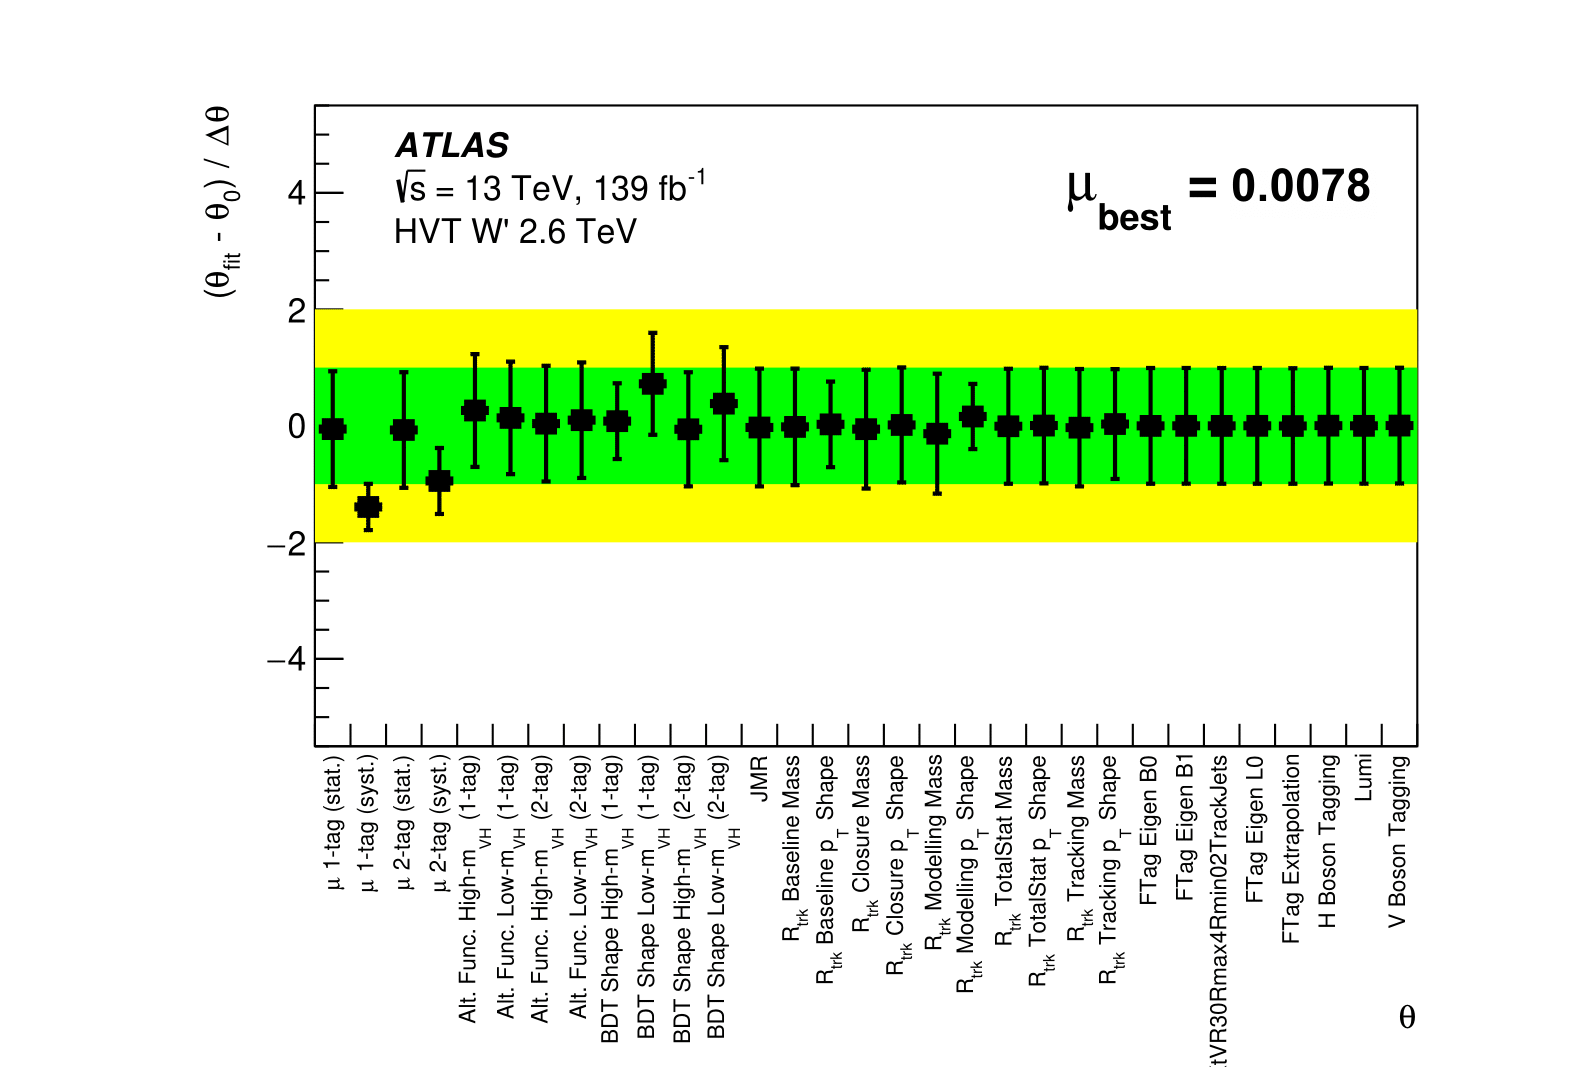
\includegraphics[width=0.7\textwidth]{Pulls_UnconditionalMu_WH_2600.png} \\
        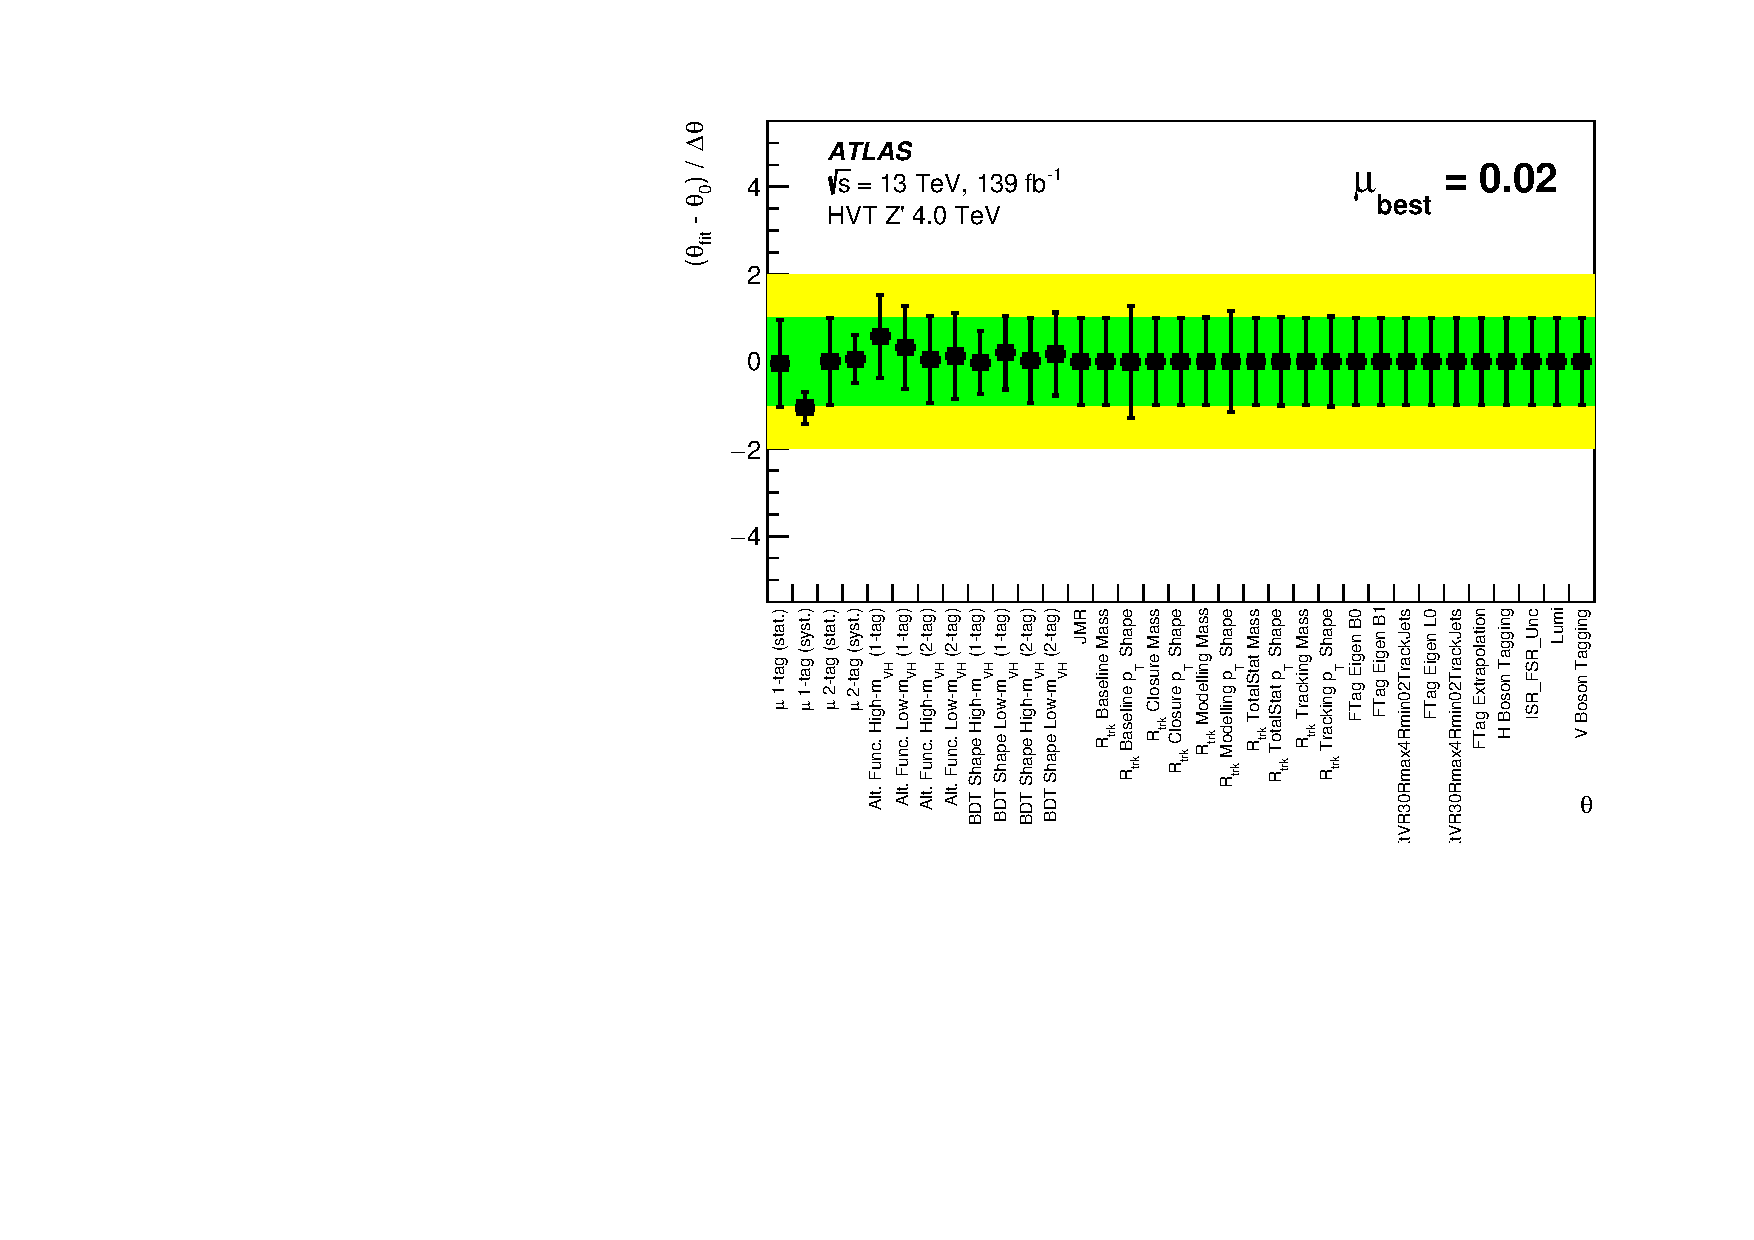
\includegraphics[width=0.7\textwidth]{Pulls_UnconditionalMu_ZH_4000.pdf}
    \end{center}
    \caption{
        Pulls and constraints on nuisance parameters in the unconstrained-$\mu$ fit (described in section \ref{sec:combined_fit}) for the 2.6 TeV WH (top) and 4.0 ZH (bottom) mass points.
    }
    \label{fig:pull_plots}
\end{figure}

\begin{figure}[htbp!]
    \begin{center}
        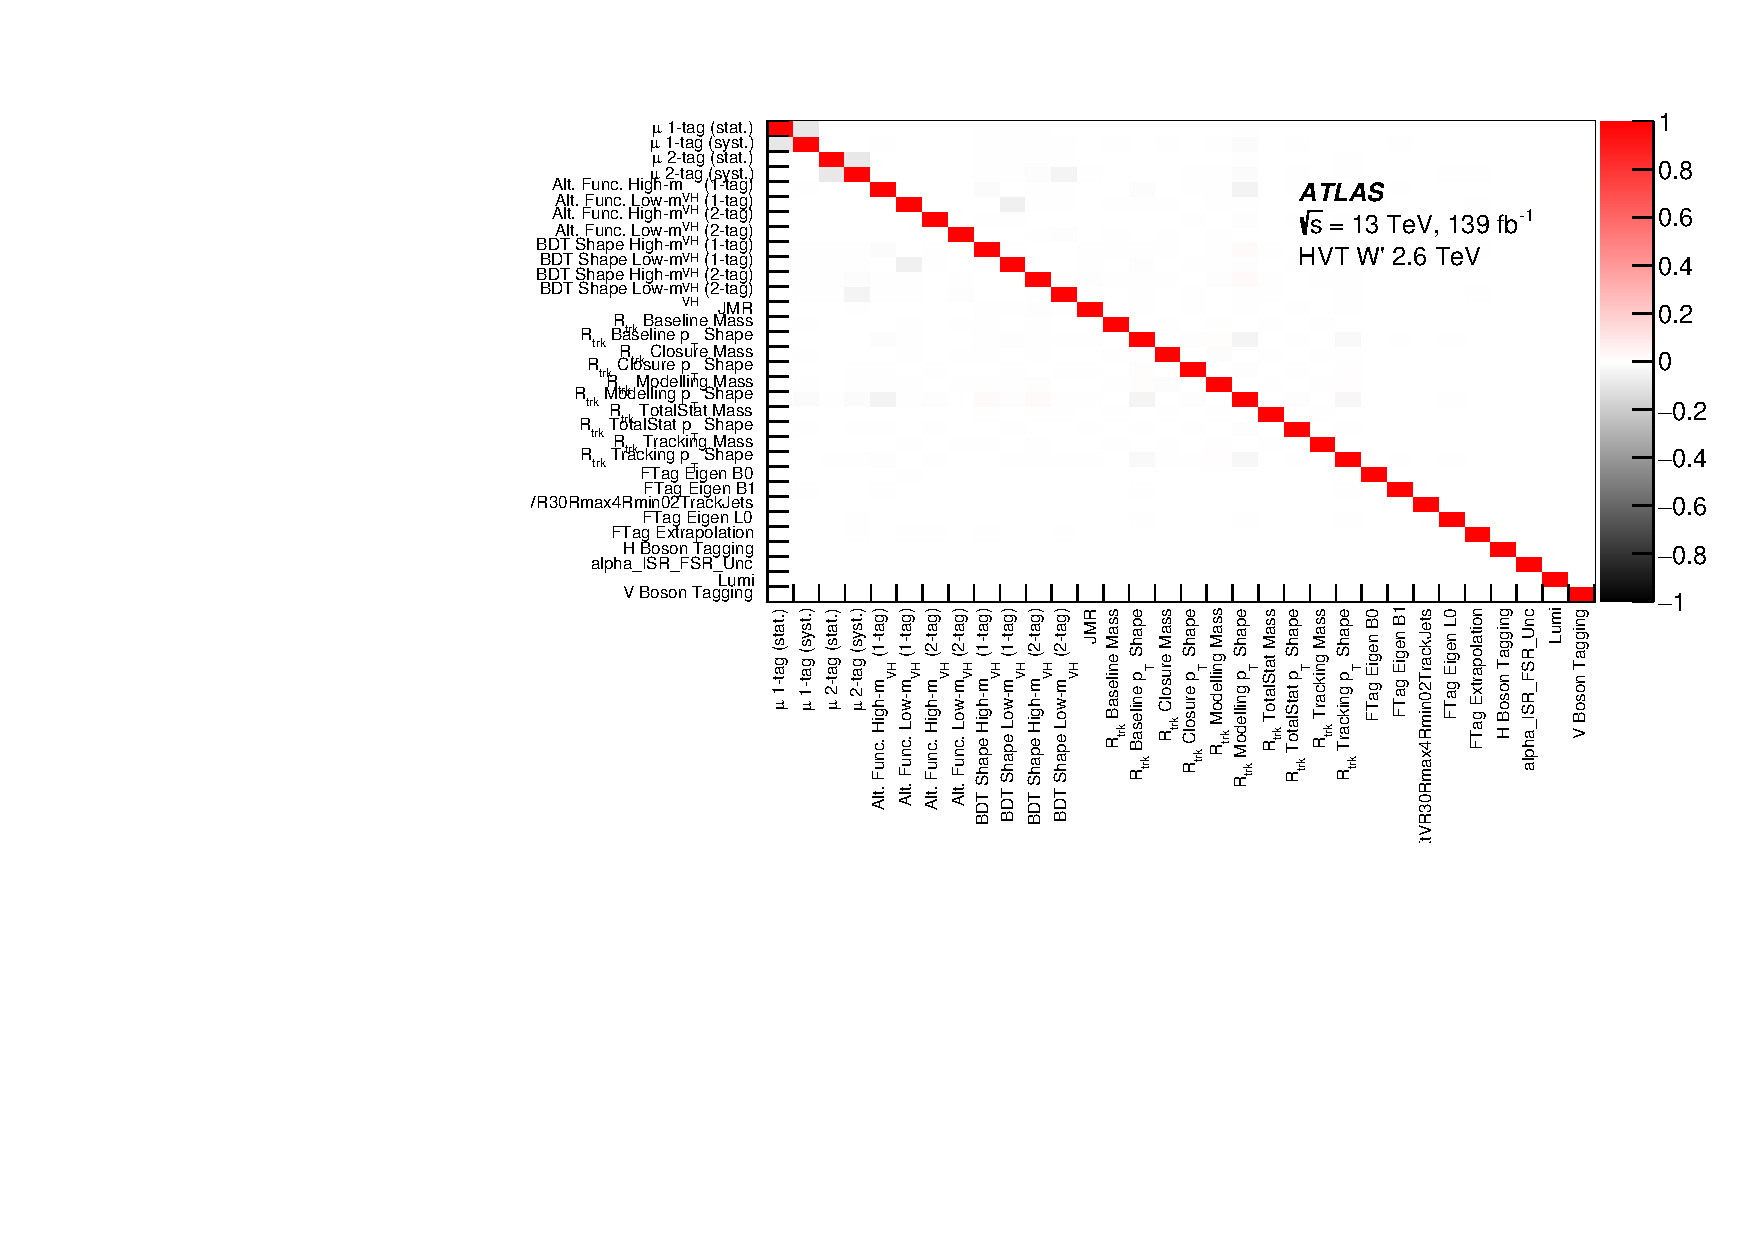
\includegraphics[width=0.7\textwidth]{CorrMatrix_UnconditionalMu_WH_2600.pdf} \\
        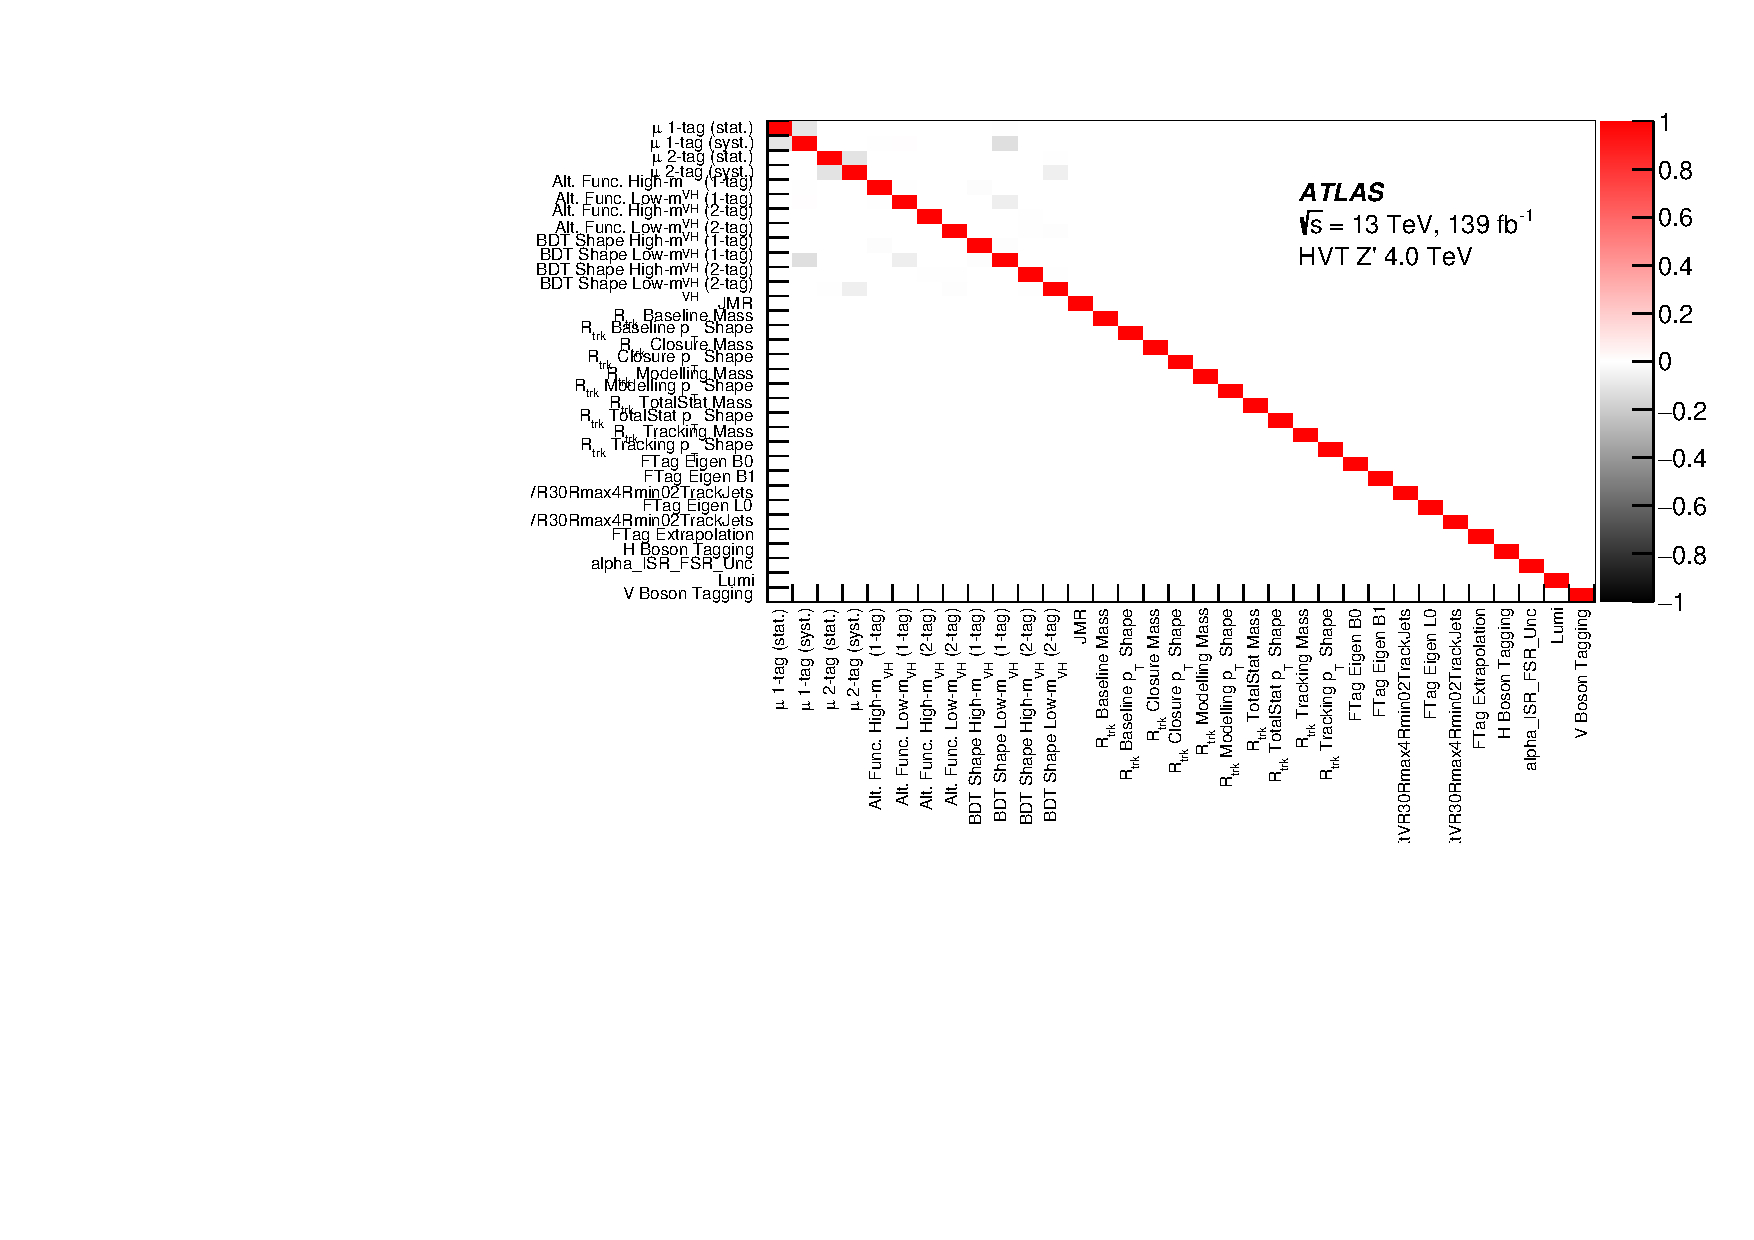
\includegraphics[width=0.7\textwidth]{CorrMatrix_UnconditionalMu_ZH_4000.pdf}
    \end{center}
    \caption{
        Correlation matrix of nuisance parameters for the 2.6 TeV (top) and 4 TeV (bottom) WH signal mass points.
    }
    \label{fig:corr_matrix_WH}
\end{figure}

\begin{figure}[htbp!]
    \begin{center}
        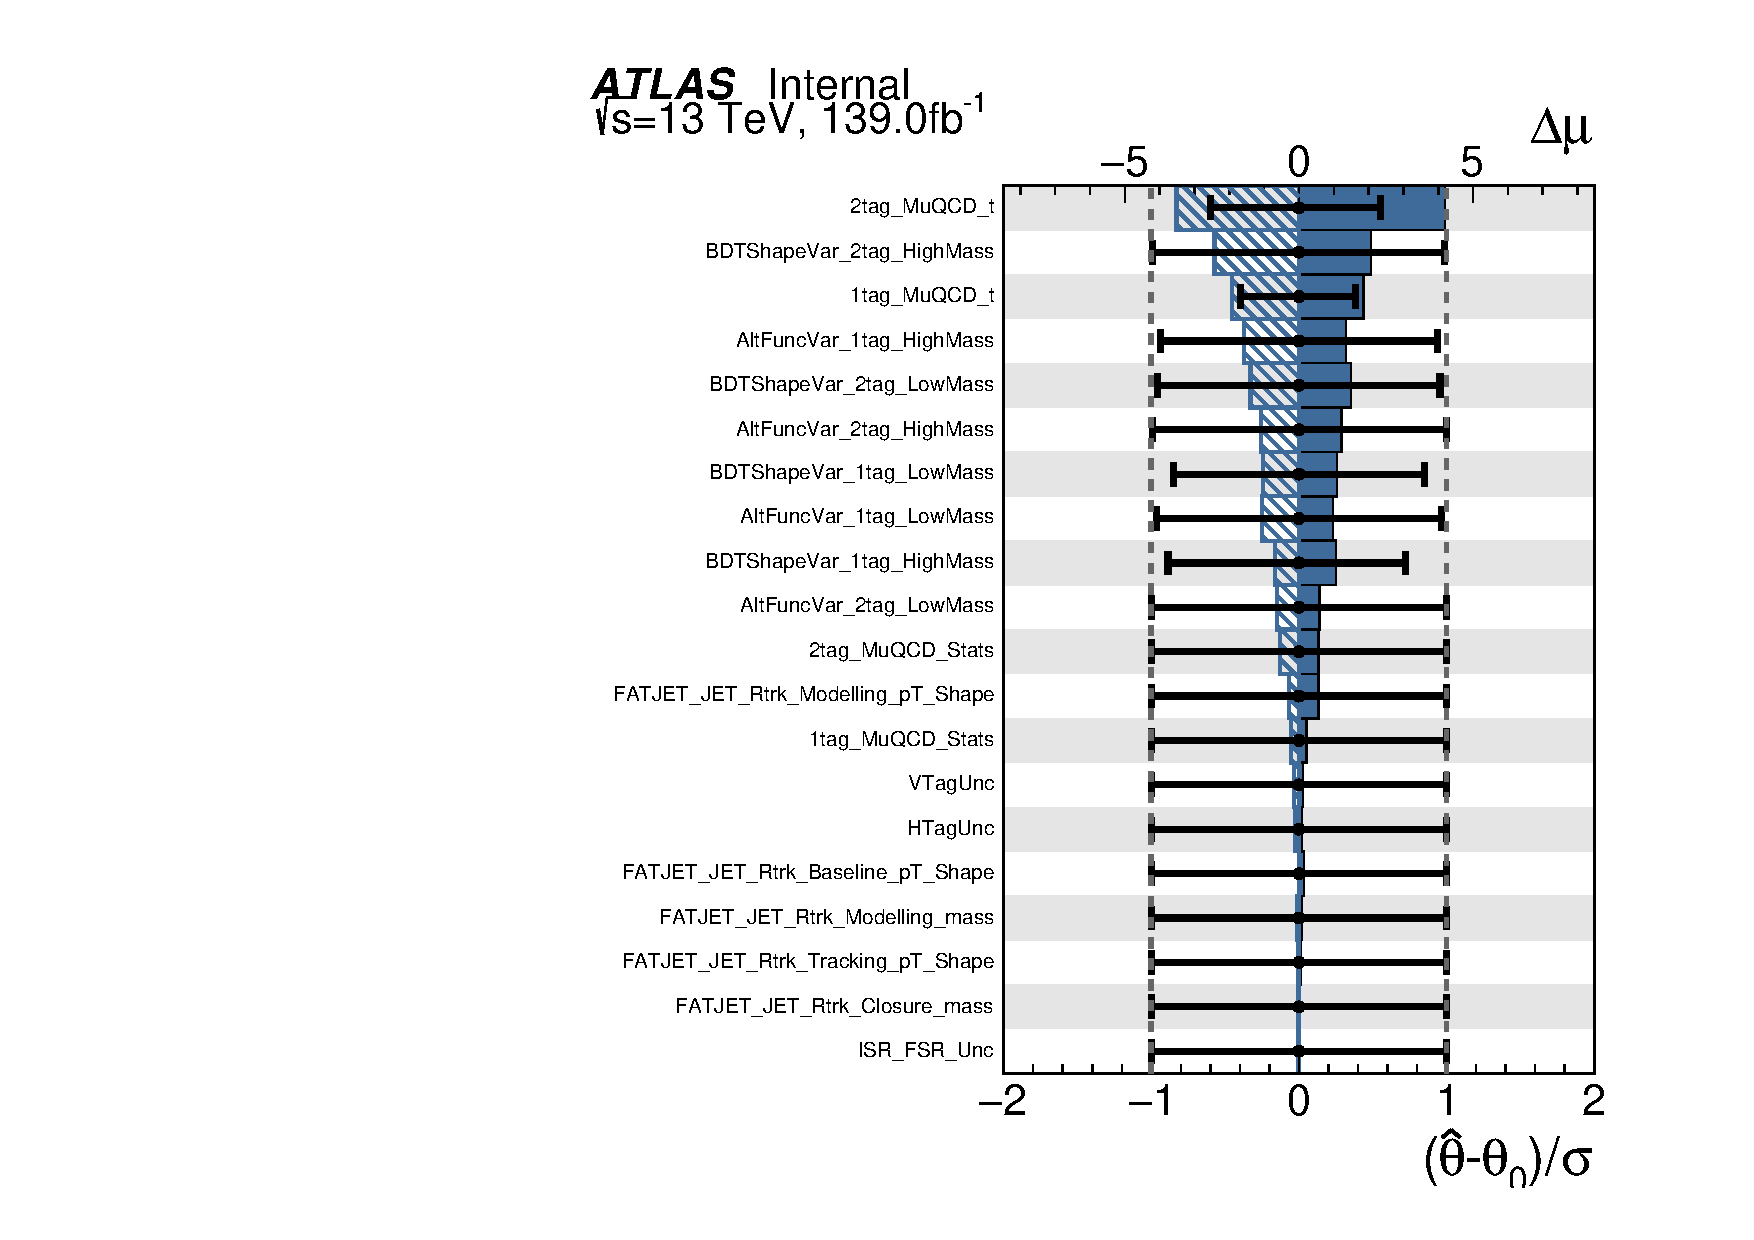
\includegraphics[width=0.49\textwidth]{Ranking_WH_2600.pdf}
        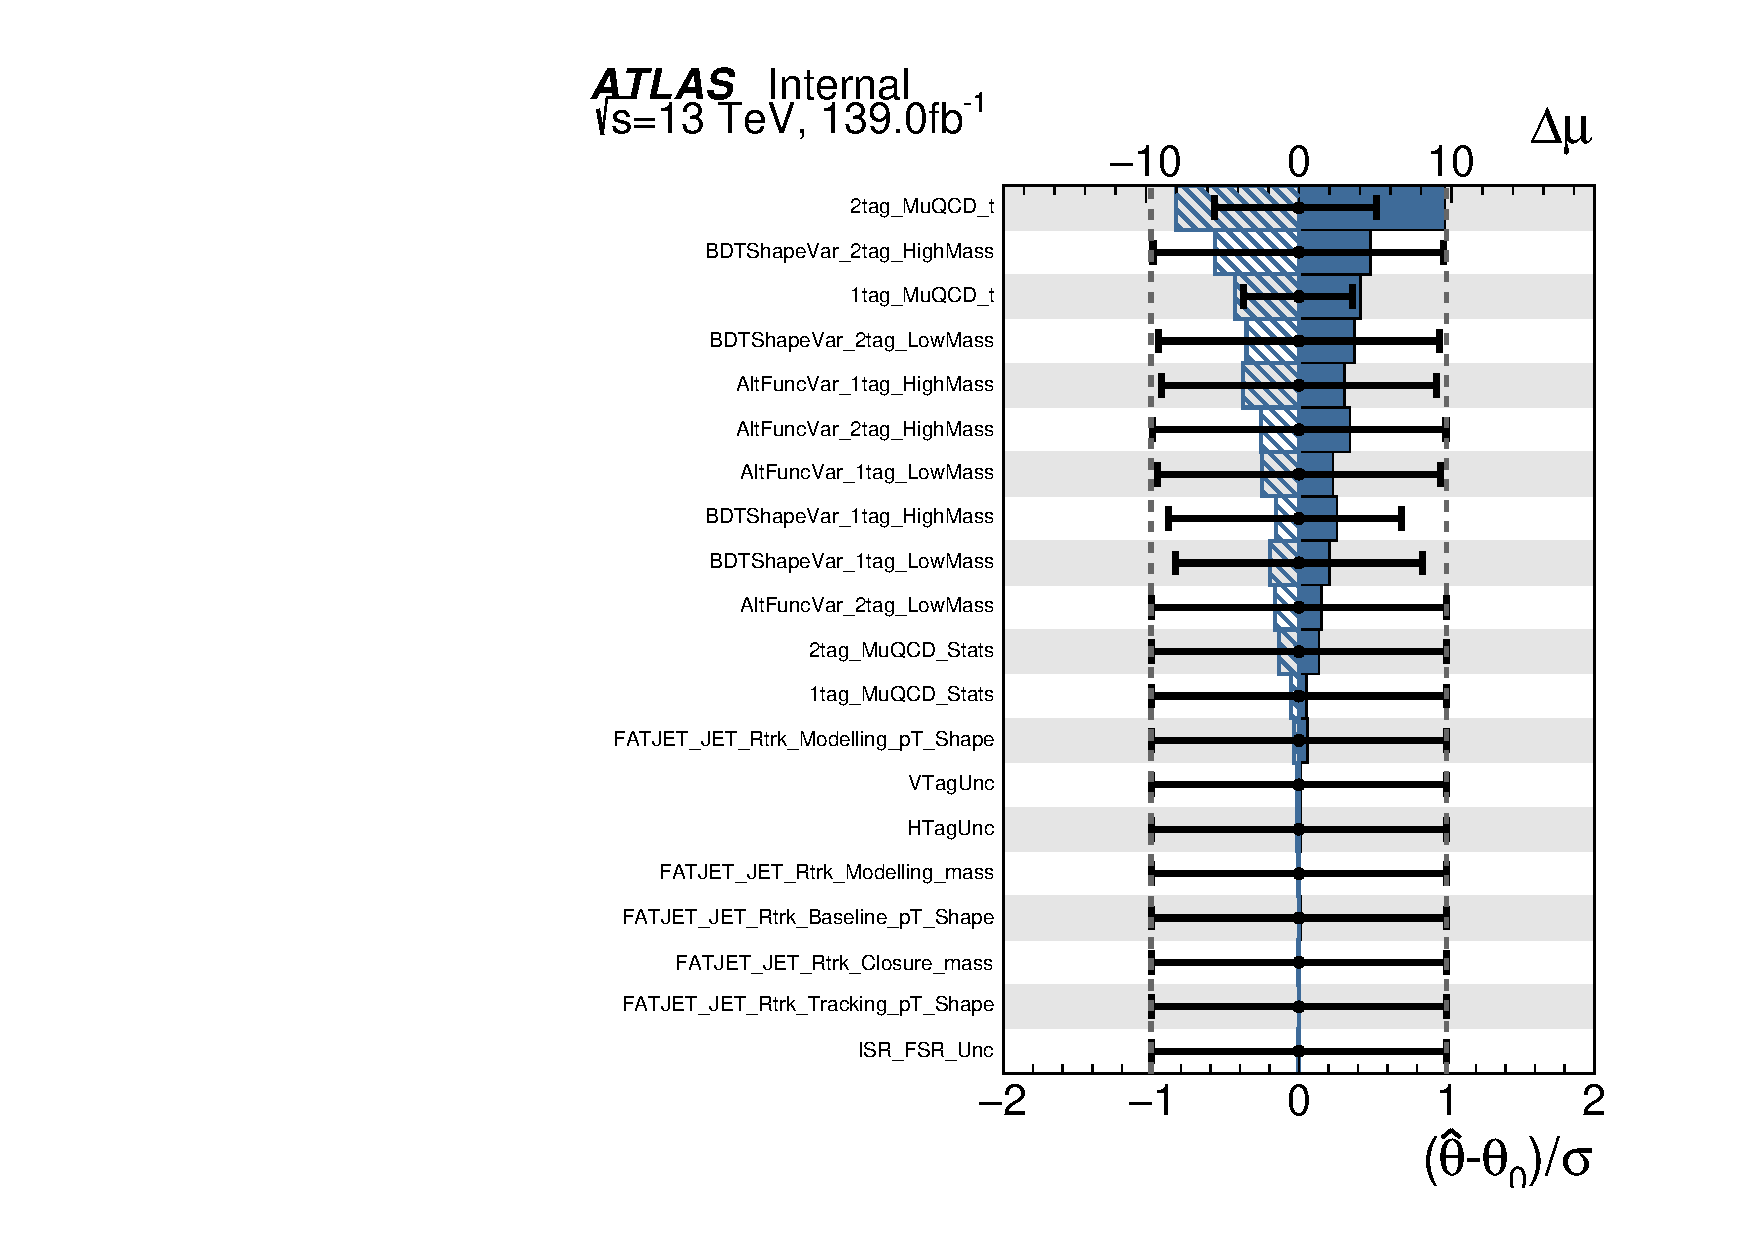
\includegraphics[width=0.49\textwidth]{Ranking_ZH_2600.pdf}
    \end{center}
    \caption{Ranking of nuisance parameters in terms of post-fit impact on $\hat{\mu}$ for the WH (left) and ZH (right) channels for the 2.6 TeV S+B fit.
        Note that the signal strength $\mu$ has been scaled by a factor of $1,000$ for purely numerical reasons.
    }
    \label{fig:rank_plots_2p6TeV}
\end{figure}

\begin{figure}[htbp!]
    \begin{center}
        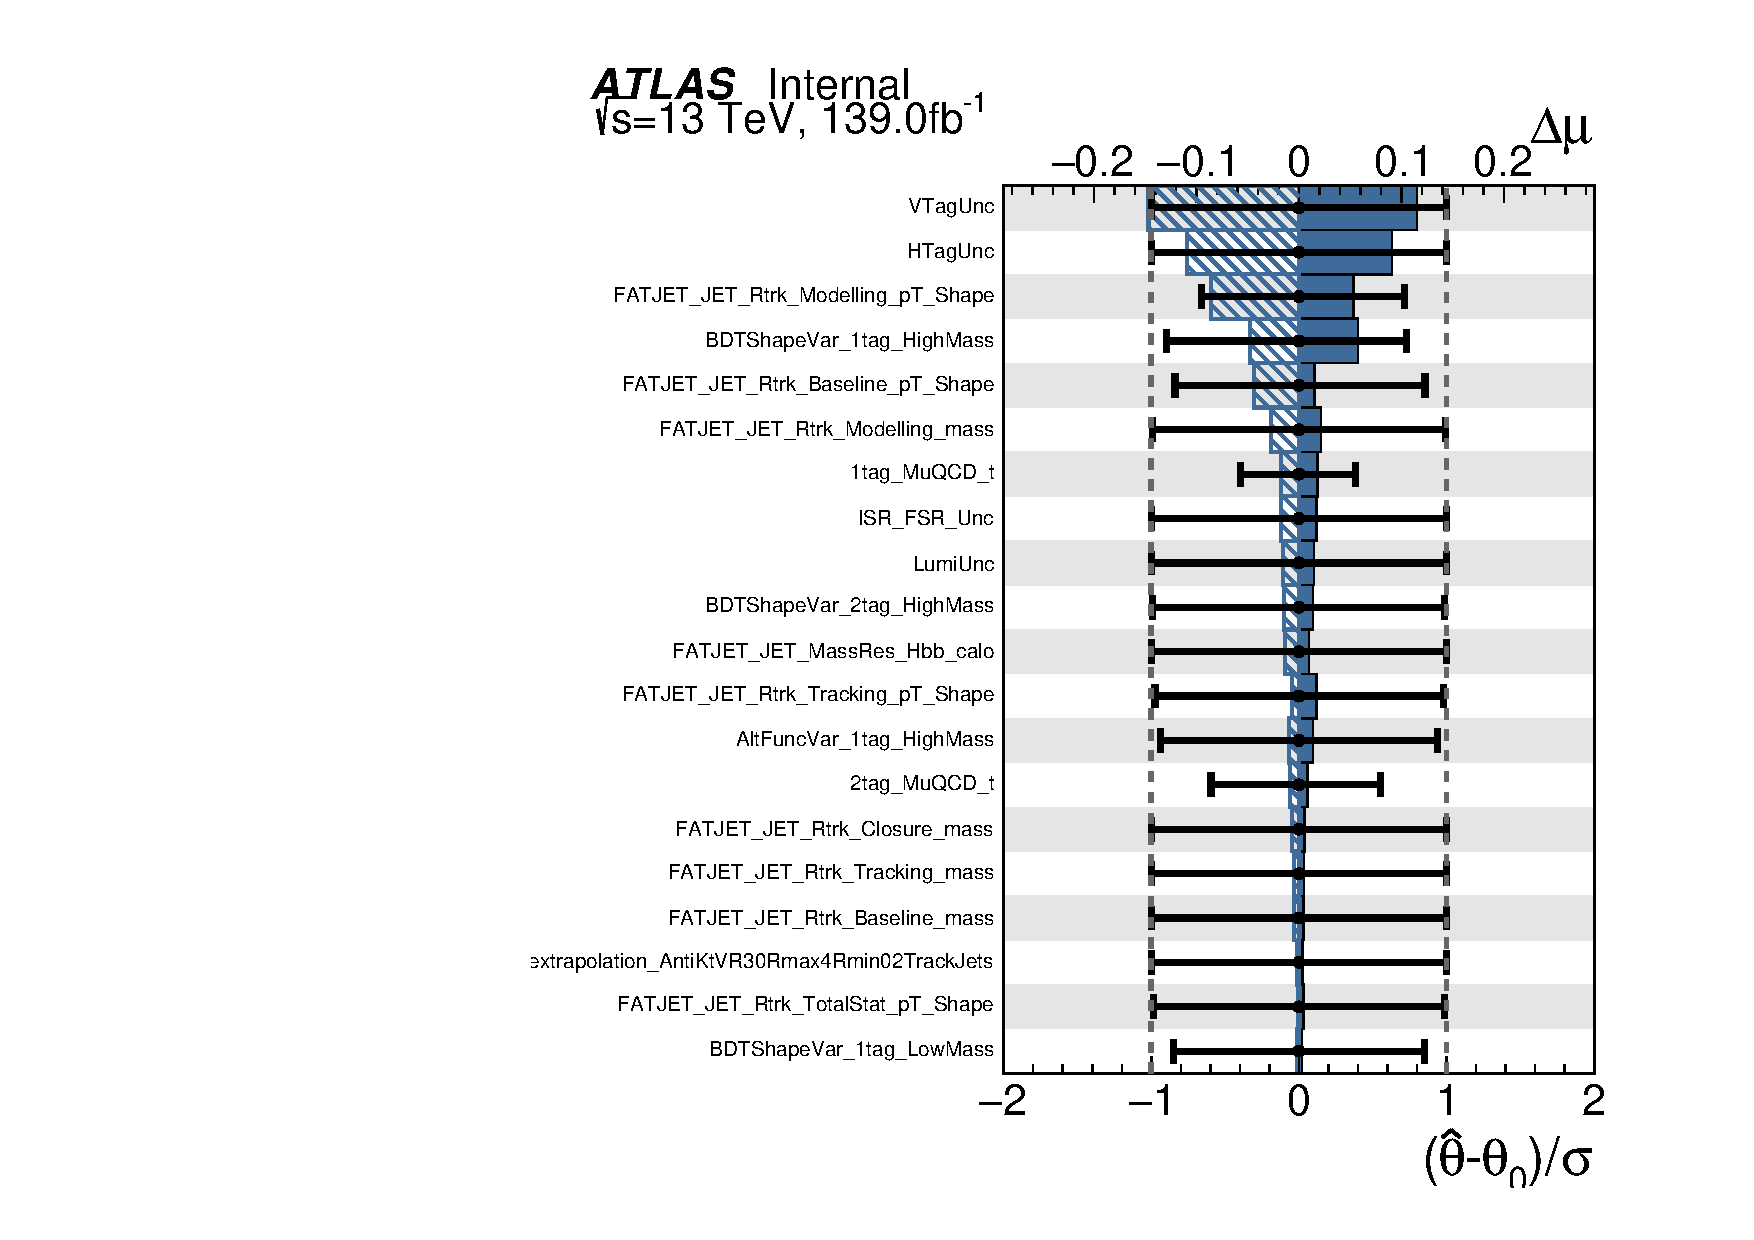
\includegraphics[width=0.49\textwidth]{Ranking_WH_4000.pdf}
        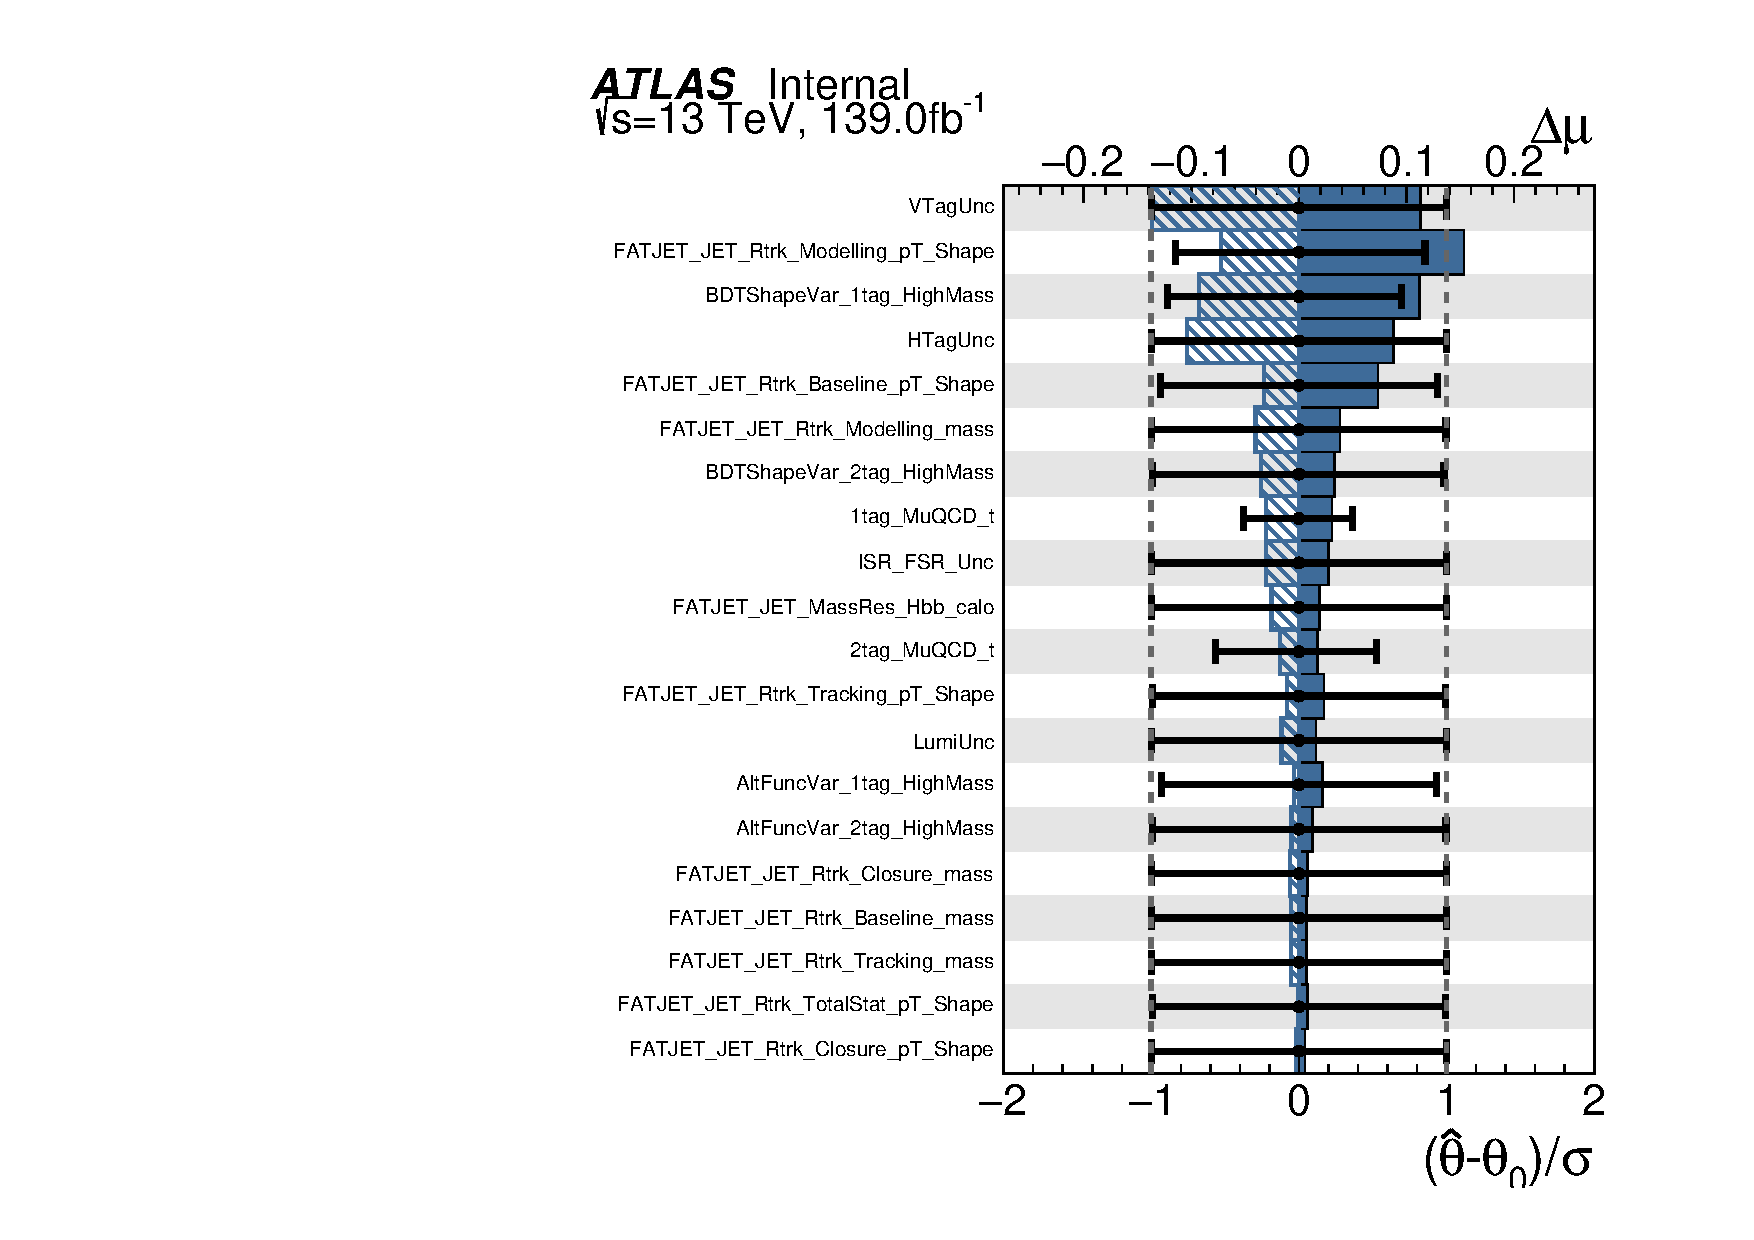
\includegraphics[width=0.49\textwidth]{Ranking_ZH_4000.pdf}
    \end{center}
    \caption{Ranking of nuisance parameters in terms of post-fit impact on $\hat{\mu}$ for the WH (left) and ZH (right) channels for the 4.0 TeV S+B fit.
    The impact on $\hat{\mu}$ is determined by repeating the combined fit with/without the nuisance parameter fixed to its nominal value and comparing the two results.
    }
    \label{fig:rank_plots_4TeV}
\end{figure}

\section{Local Significance}

The relevance of any excesses observed in data with respect to the background expectation is quantified by estimating the local signifiance ($p_0$) using the asymptotic approximation.
The combined local significance of the 1-tag + 2-tag channels is shown for both WH and ZH samples in Figure~\ref{fig:local_p0_combined}.
The largest deviation is observed in the fit to the WH signal region and corresponds to a $p_0$ value of 0.03 for a resonance mass of 2.8 TeV.

\begin{figure}[htbp!]
    \begin{center}
        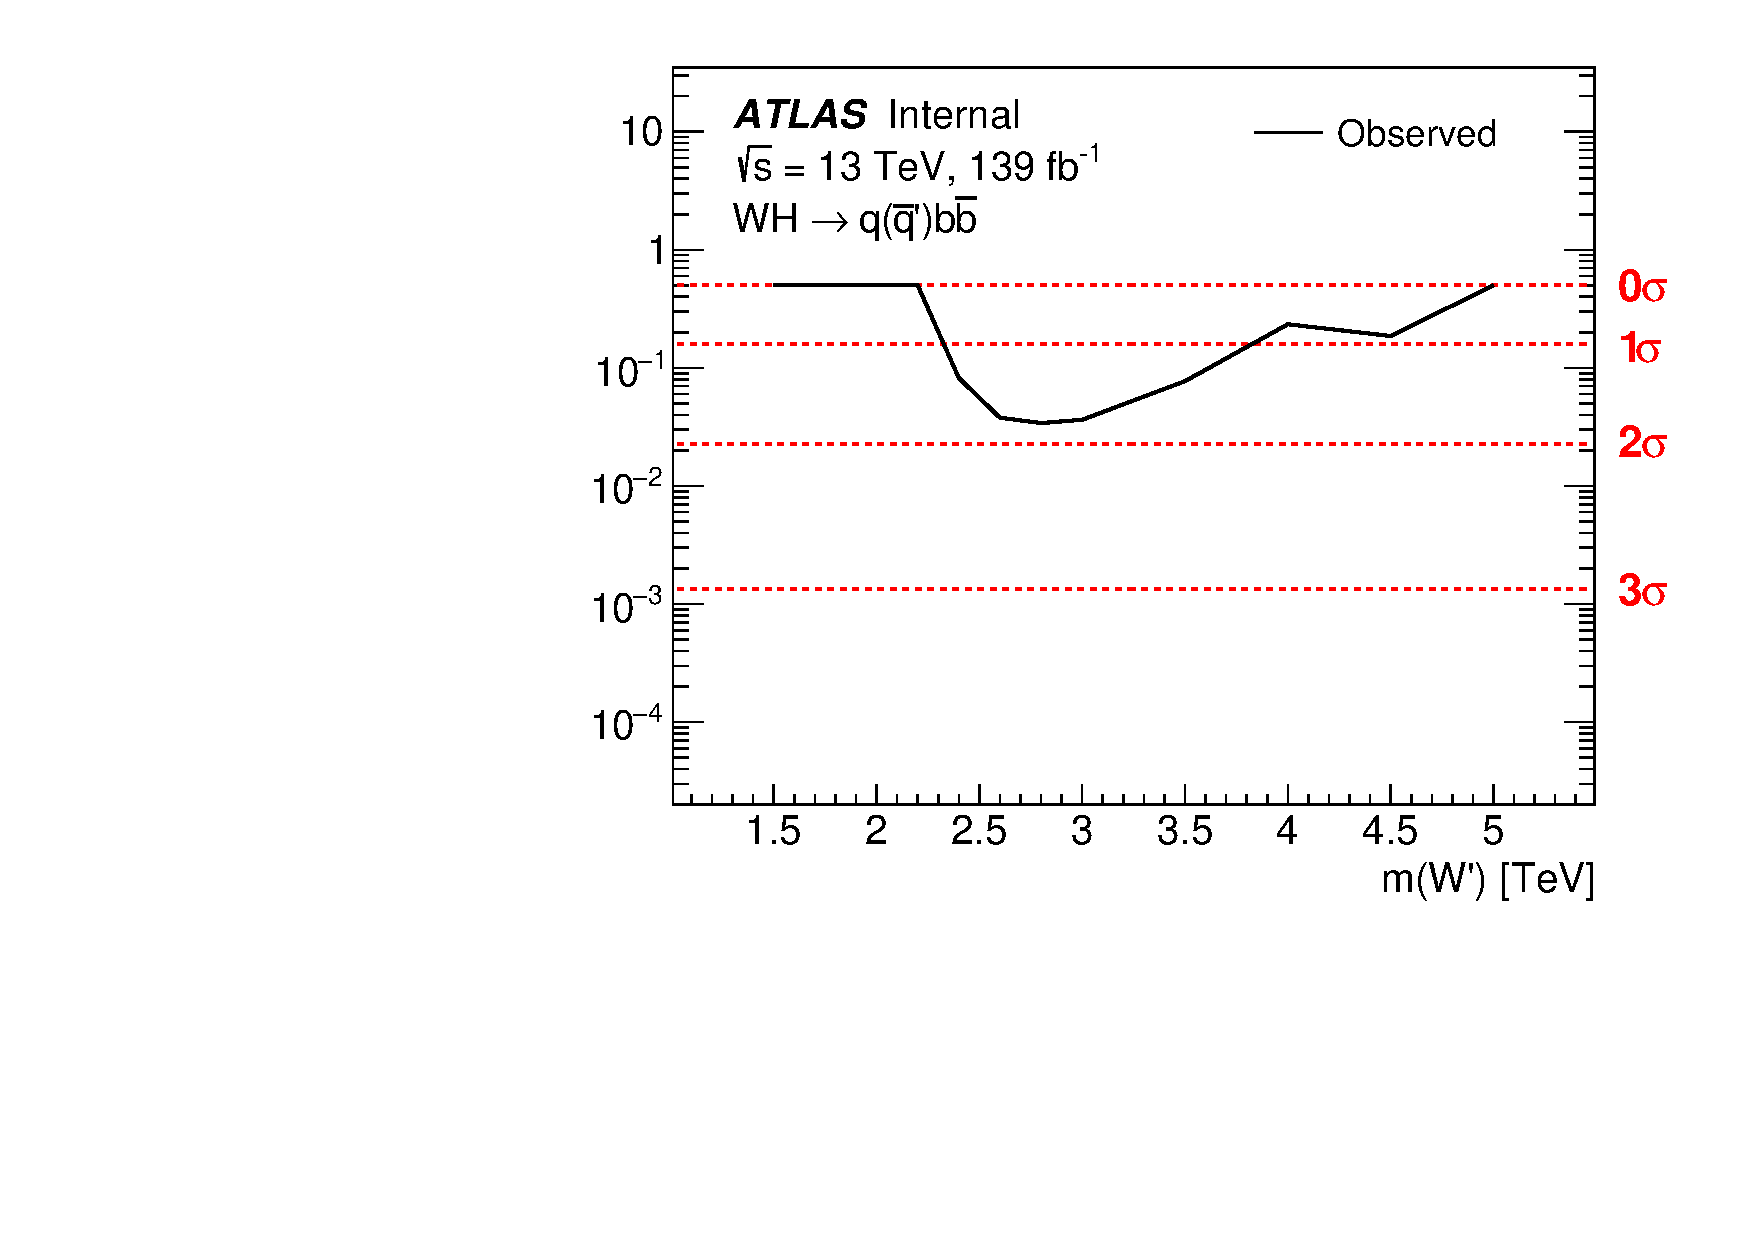
\includegraphics[width=0.49\textwidth]{VHqqbbLocalP0_WH.pdf}
        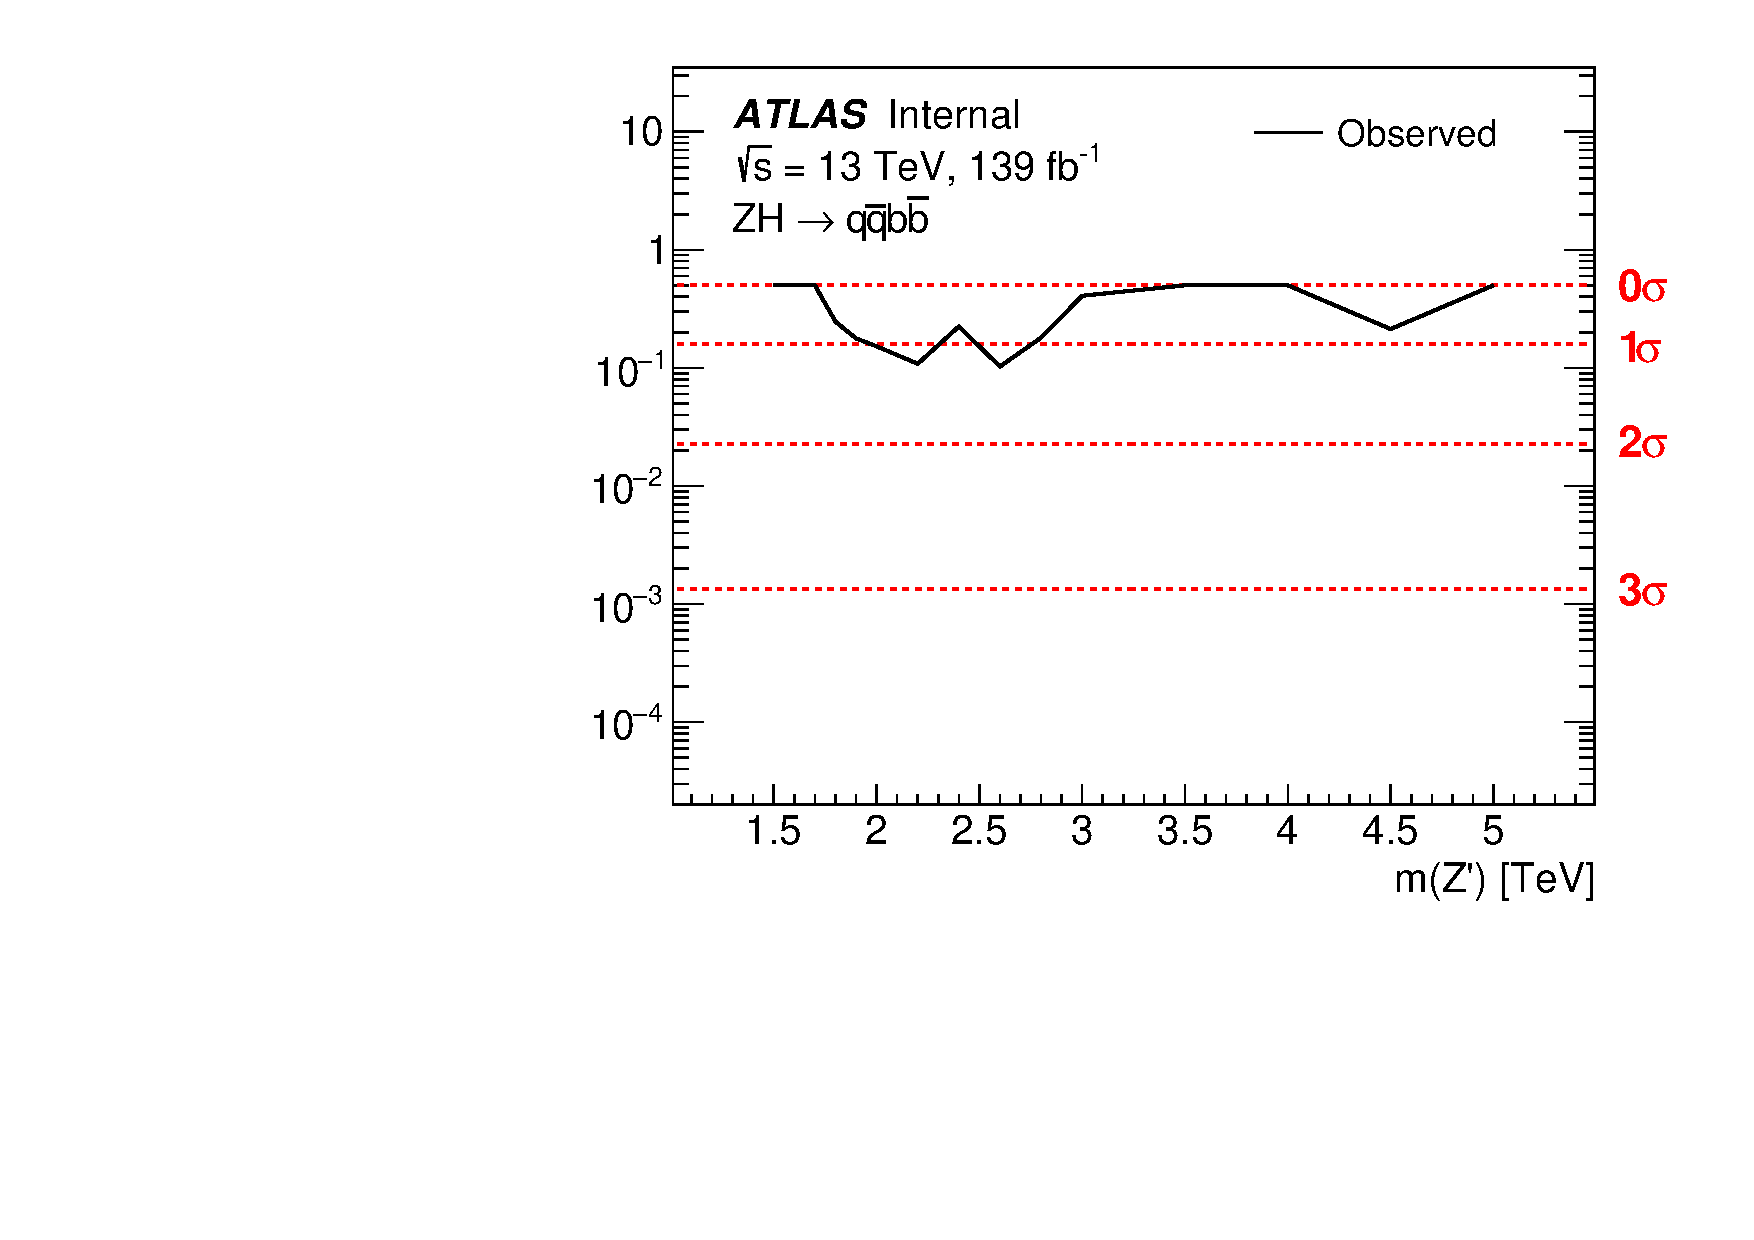
\includegraphics[width=0.49\textwidth]{VHqqbbLocalP0_ZH.pdf}
    \end{center}
    \caption{Observed local $p_0$ values for the combined 1-tag + 2-tag WH (left) and ZH (right) channels.}
    \label{fig:local_p0_combined}
\end{figure}

\section{Upper Limits on Cross Section}
Upper limits on the cross section times branching ratio for a resonance decaying to $VH$ are shown in Figure~\ref{fig:exp_limits_atlas}, for both the WH and ZH signal regions.
The expected and observed upper limits are compared to the predictions for HVT Models A and B, from which mass exclusion values can be determined.
For Model A, the excluded signal mass ranges are 1500-2900 GeV for $WH$ resonances, and 1500-2200 GeV for $ZH$ resonances.
For Model B, the excluded signal mass ranges are 1500-3200 GeV for $WH$ resonances, and 1500-2650 GeV for $ZH$ resonances.
These results can also be translated into exclusions in the {$g_H,g_f$} plane, where $g_f$ represents a universal coupling between the $V'$ bosons and fermions.
Here, $g_q$ is taken to be equal to $g_f$. Figure ~\ref{fig:hvt_coupling_plane} shows the 95\% CL limits in this plane for several resonance masses.
The individual contributions from the separate 1/2-tag channels are shown in Figure ~\ref{fig:exp_limit_channels}.
The expected limits at 95\% confidence level are compared to the previous iteration of the analysis in Figure~\ref{fig:exp_limit_cmp}.
The results presented in this thesis are the strongest constraints to date.
The primary sources of improvement in this result are the re-optimized boson tagging criteria, the inclusion of the $n_{\mathrm{trk}}$ variable for $W$/$Z$ tagging, the use of VR track jets instead of fixed radius track jets, and the improved background prediction strategy utilizing BDT-reweighting and improved binning/smoothing.

\begin{figure}[htbp!]
    \begin{center}
        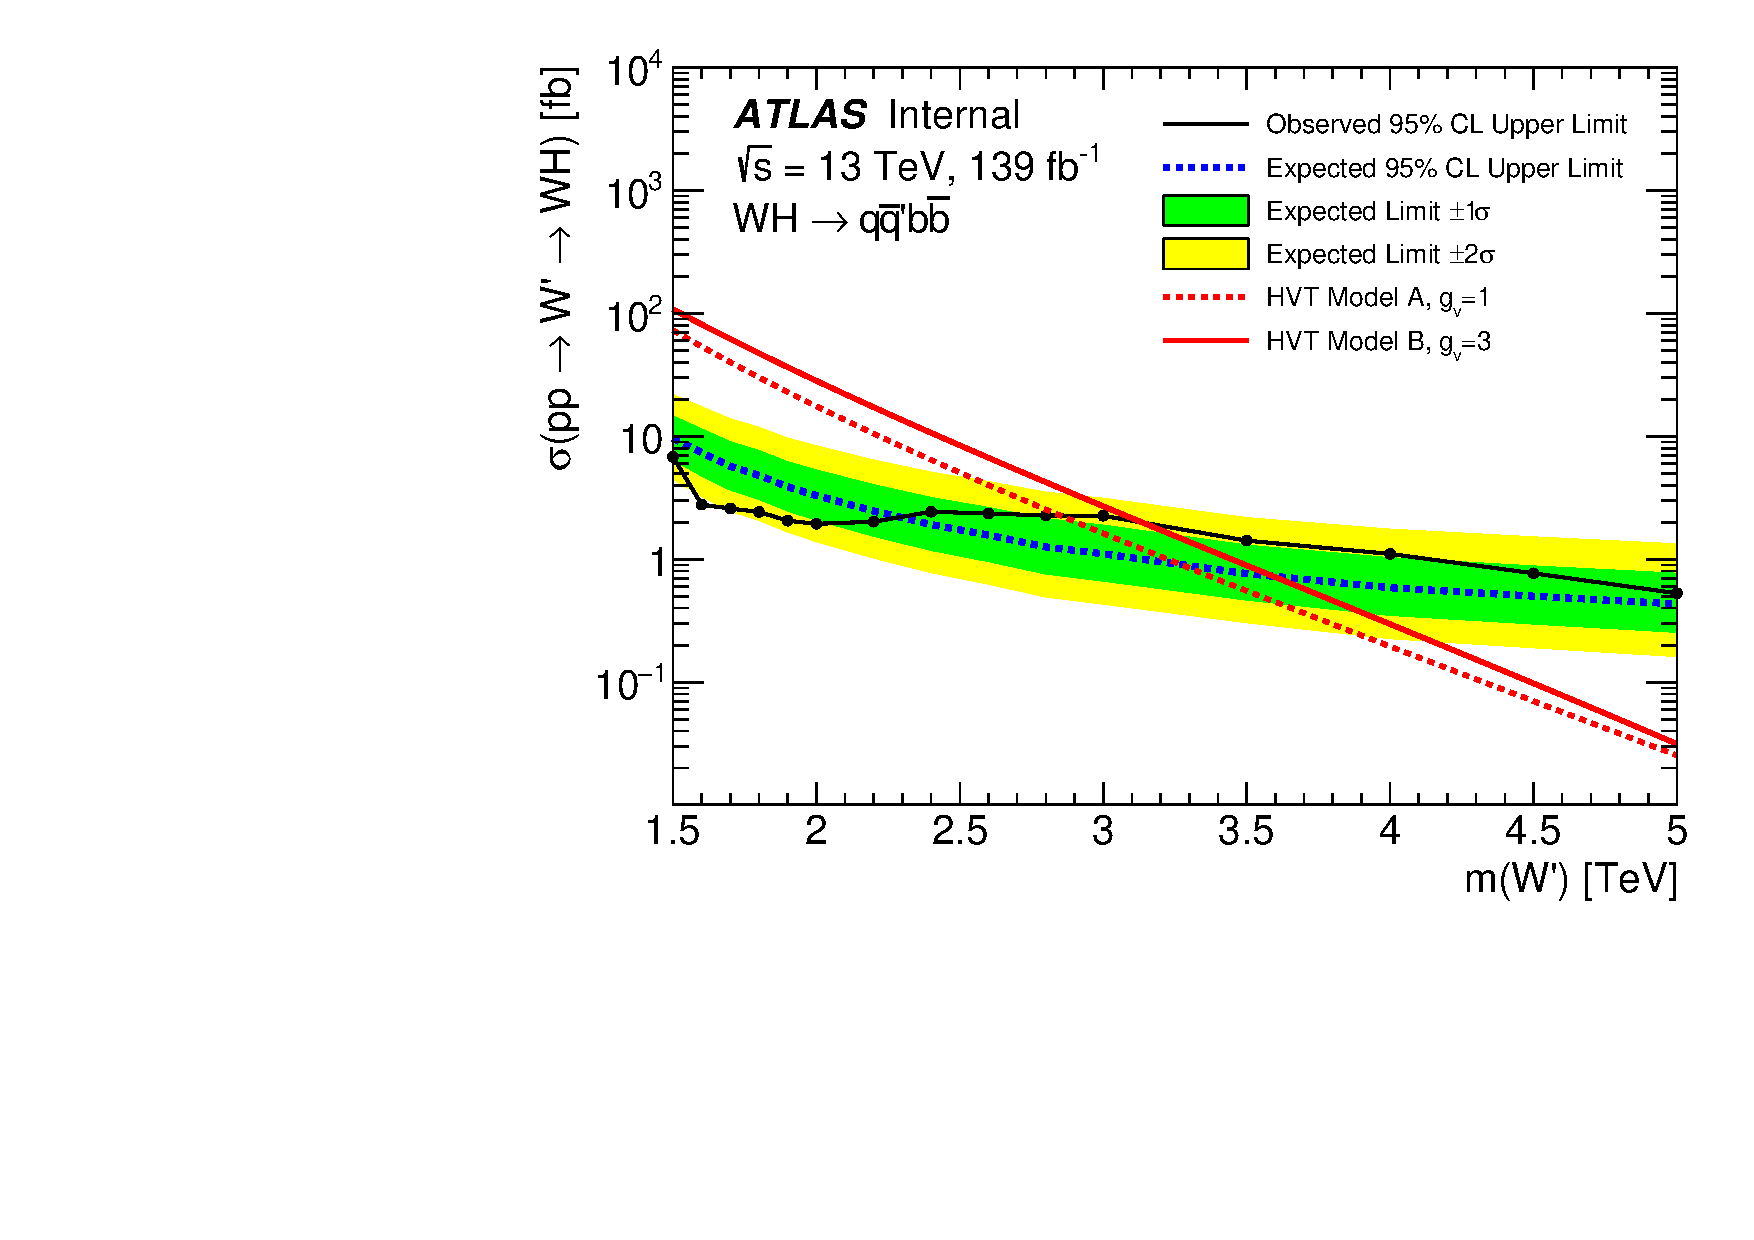
\includegraphics[width=0.49\textwidth]{VHqqbbLimitATLAS_WH.pdf}
        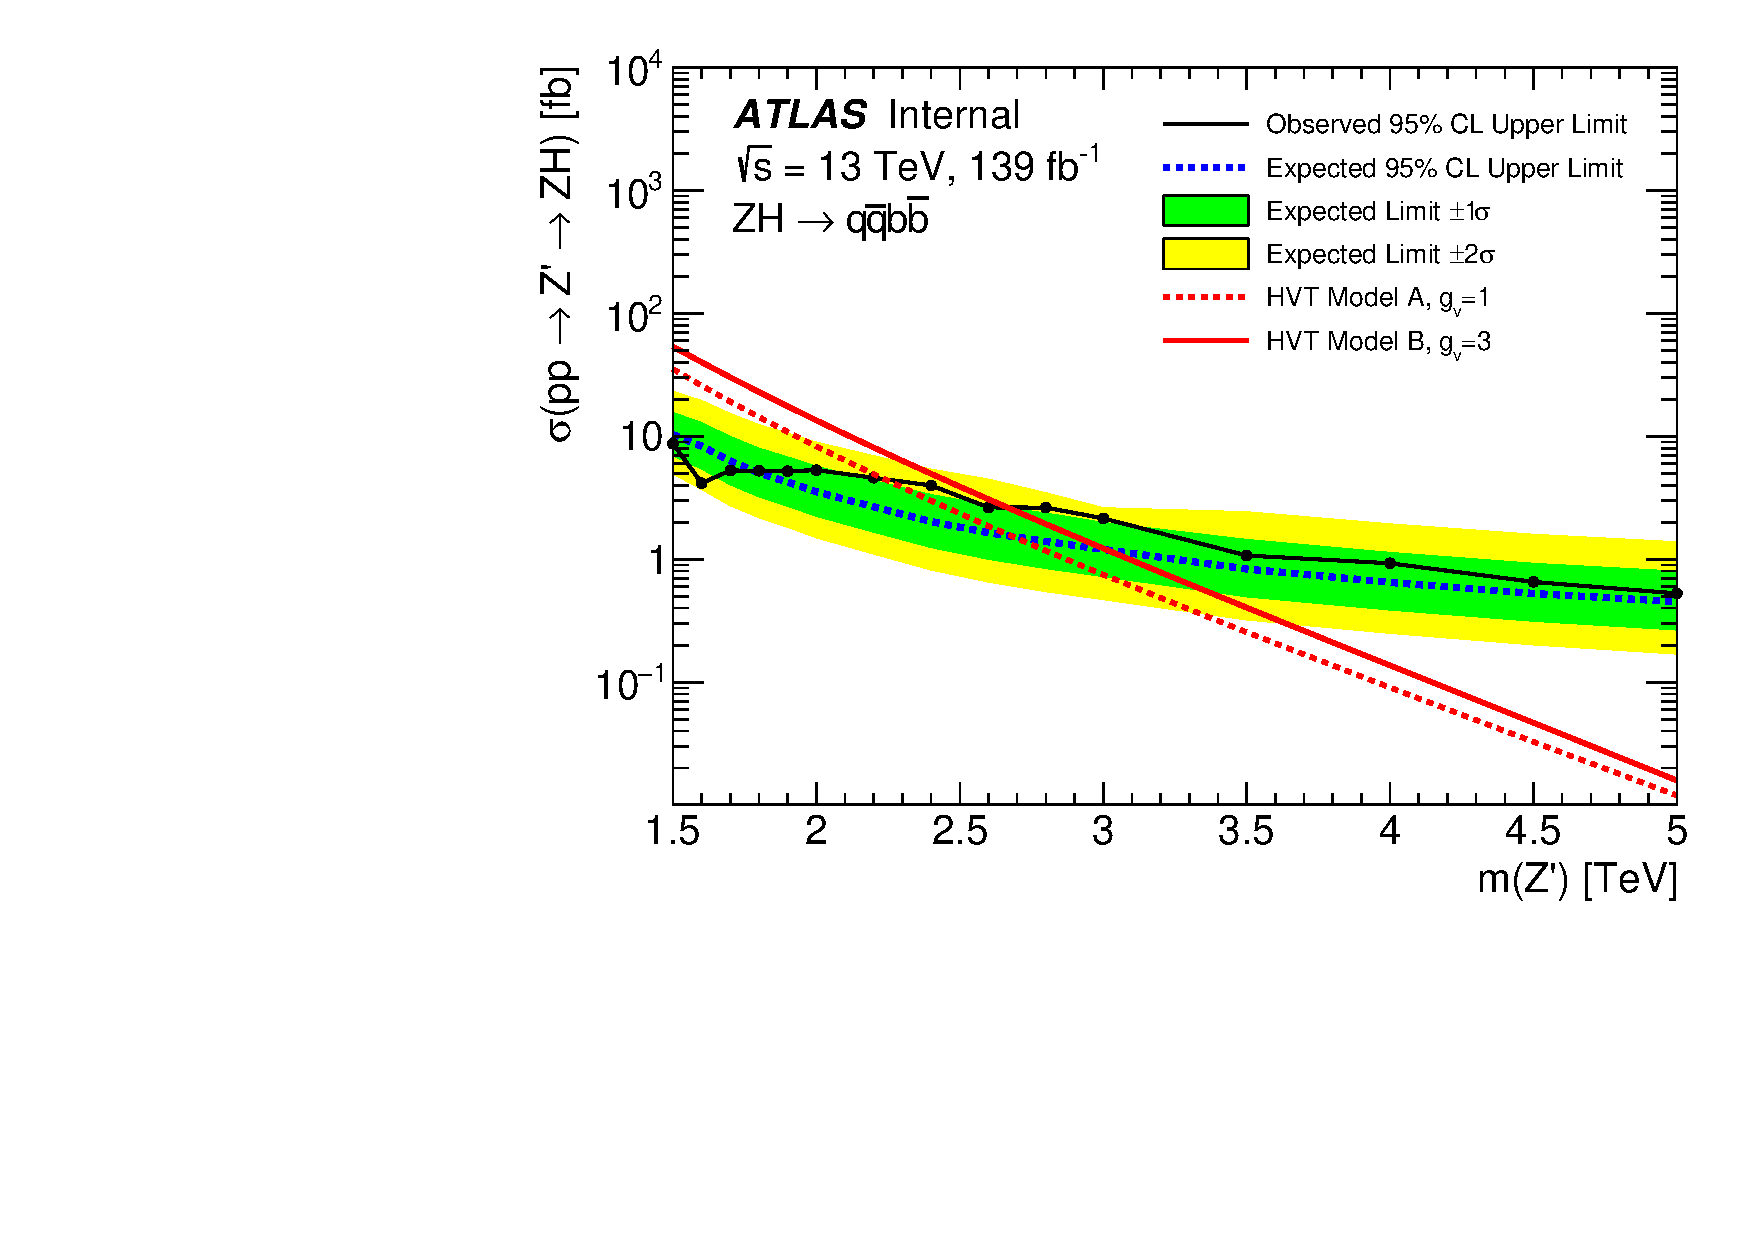
\includegraphics[width=0.49\textwidth]{VHqqbbLimitATLAS_ZH.pdf}
    \end{center}
    \caption{Upper limits on $\sigma(V^\prime \rightarrow VH)$ at 95\% CL for WH (left) and ZH (right) channels.
        The figures show the expected limits and predicted cross sections for the HVT Models A and B.
    }
    \label{fig:exp_limits_atlas}
\end{figure}

\begin{figure}[htbp!]
    \begin{center}
        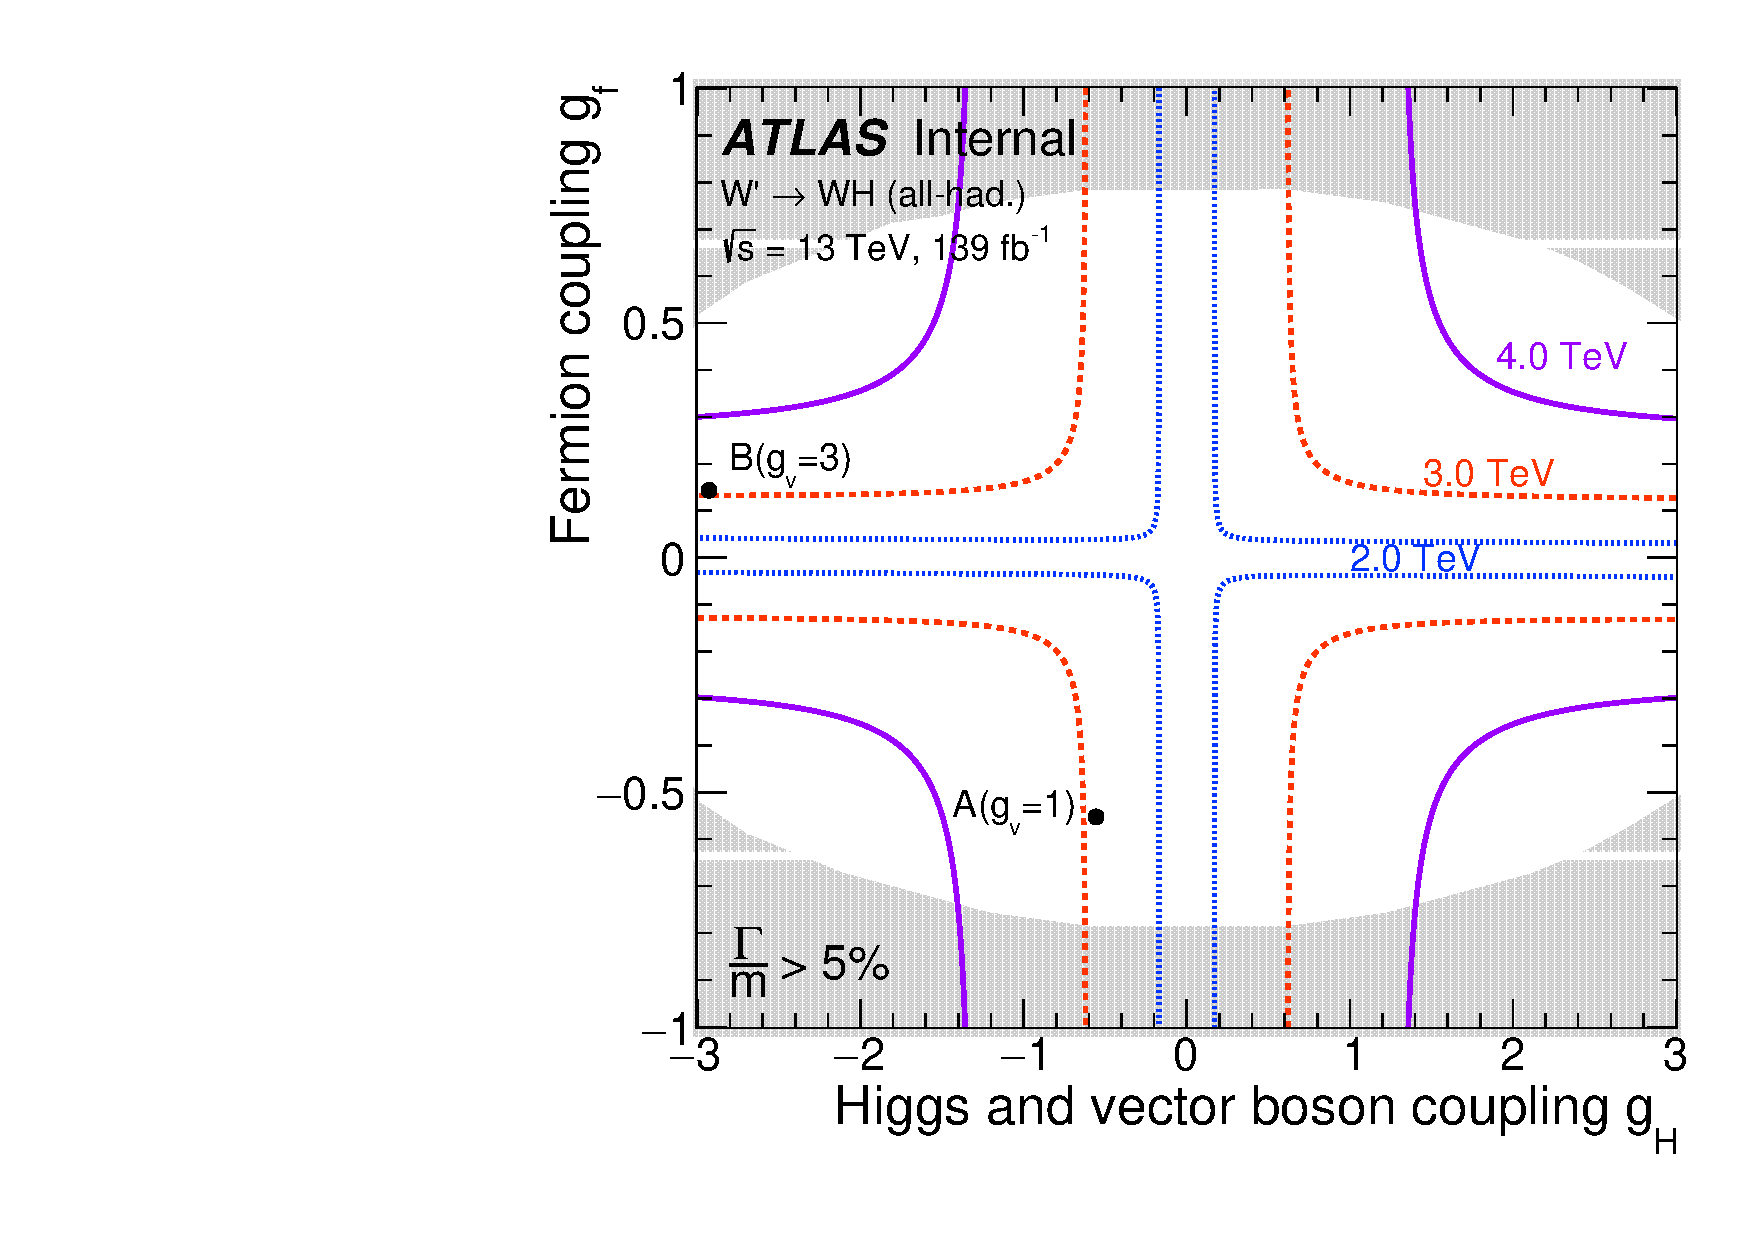
\includegraphics[width=0.49\textwidth]{HVT_coupling_WH.pdf}
        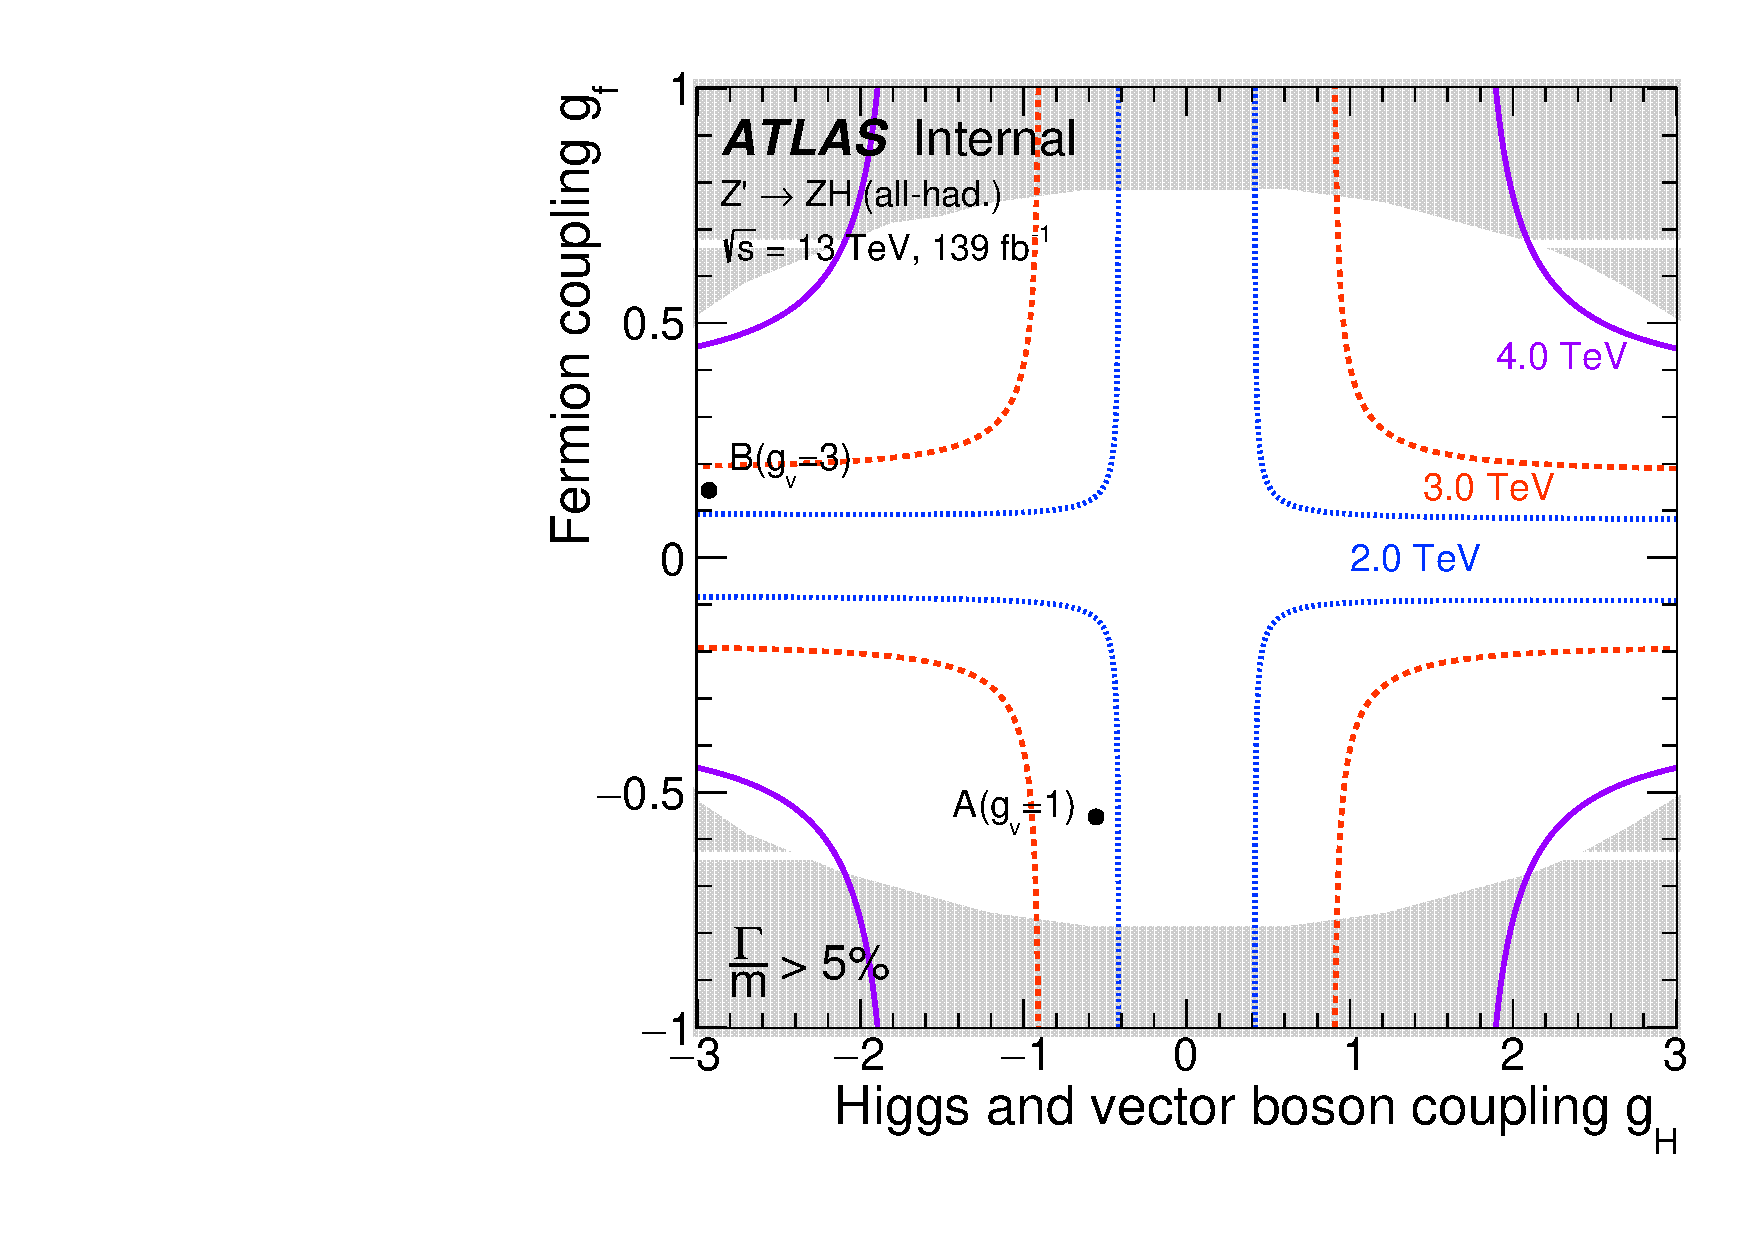
\includegraphics[width=0.49\textwidth]{HVT_coupling_ZH.pdf}
    \end{center}
    \caption{
        Limits in the $g_f$ vs. $g_H$ coupling plane for resonance masses of 2, 3, and 4 TeV for the WH (left) and ZH (right) channels in the context of the HVT model.
        The coupling values corresponding to the HVT models A and B are indicated by filled circles.
    }
    \label{fig:hvt_coupling_plane}
\end{figure}

\begin{figure}[htbp!]
    \begin{center}
        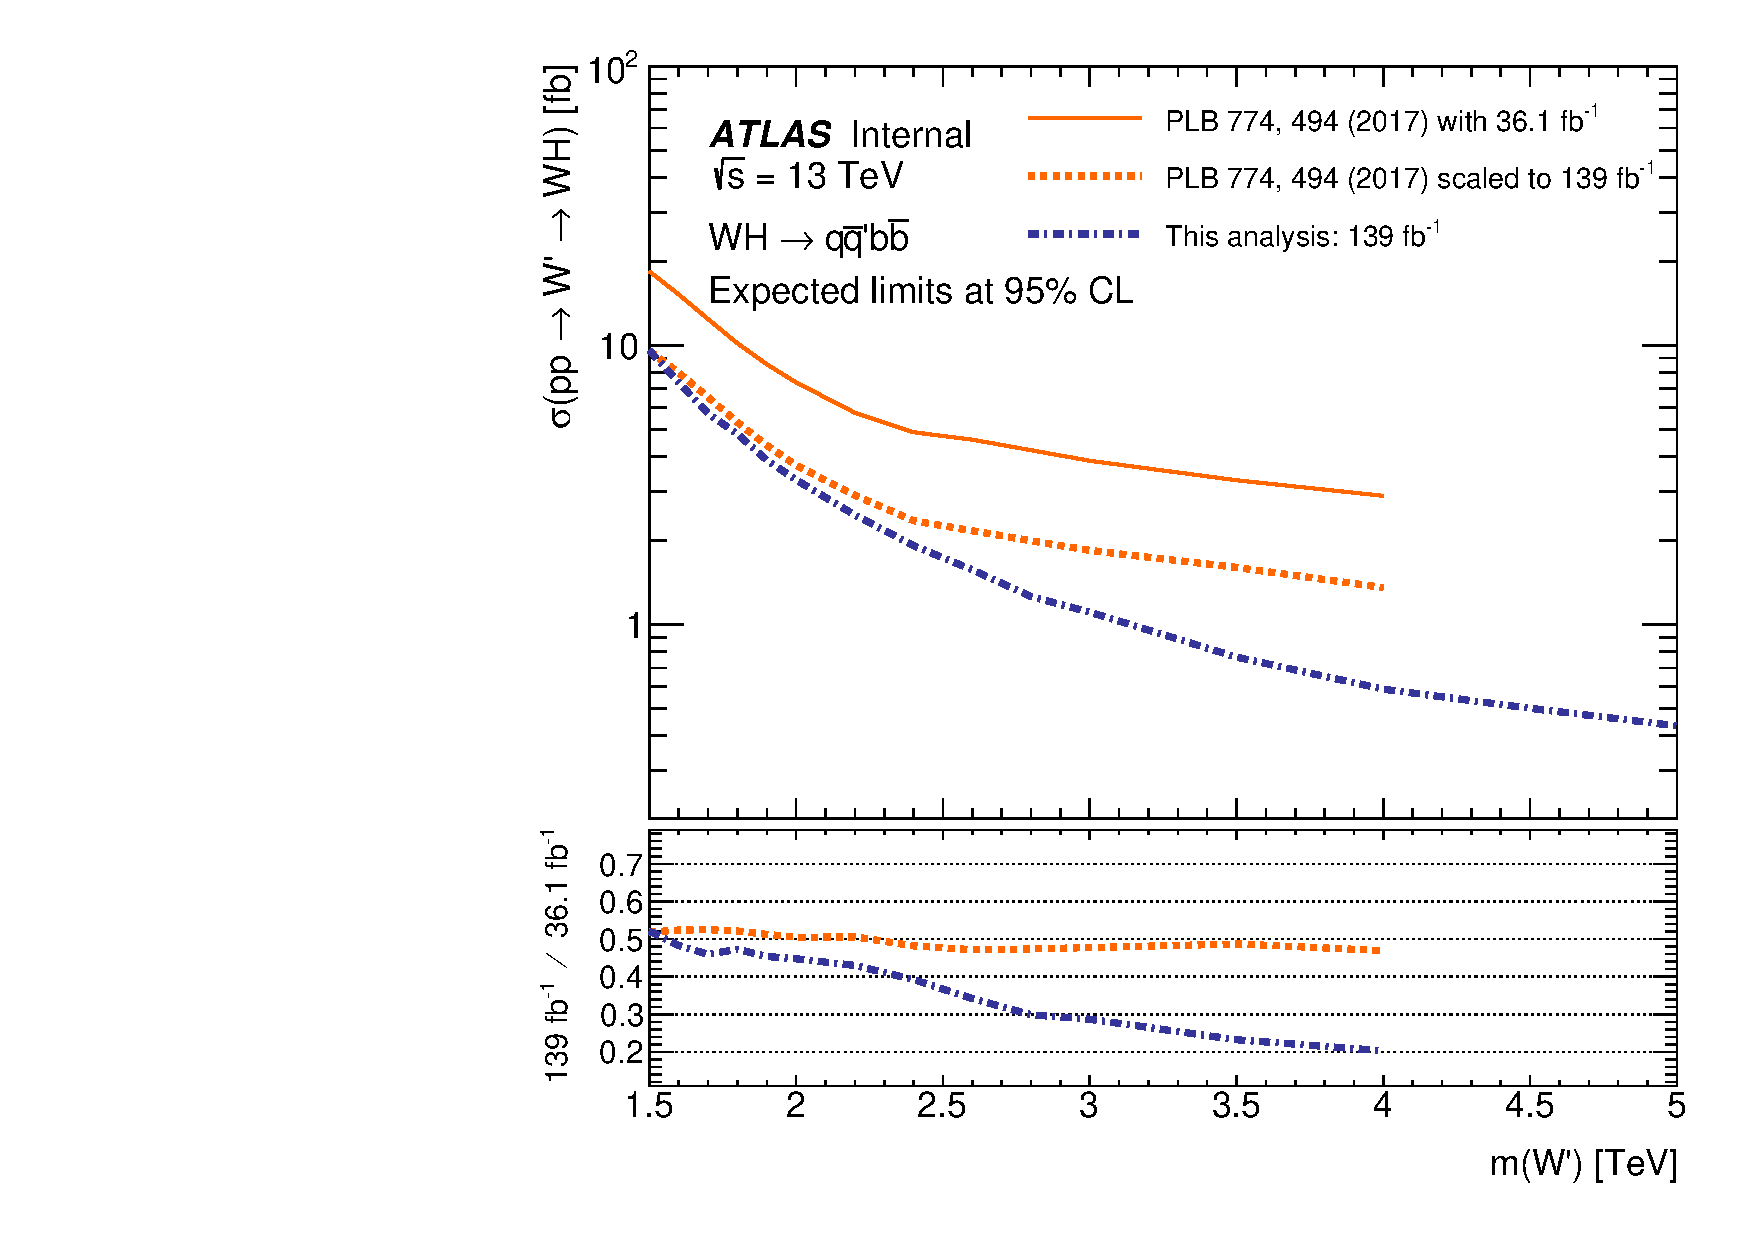
\includegraphics[width=0.65\textwidth]{VHqqbbLimit_WH_2016_2019_v4.pdf} \\
        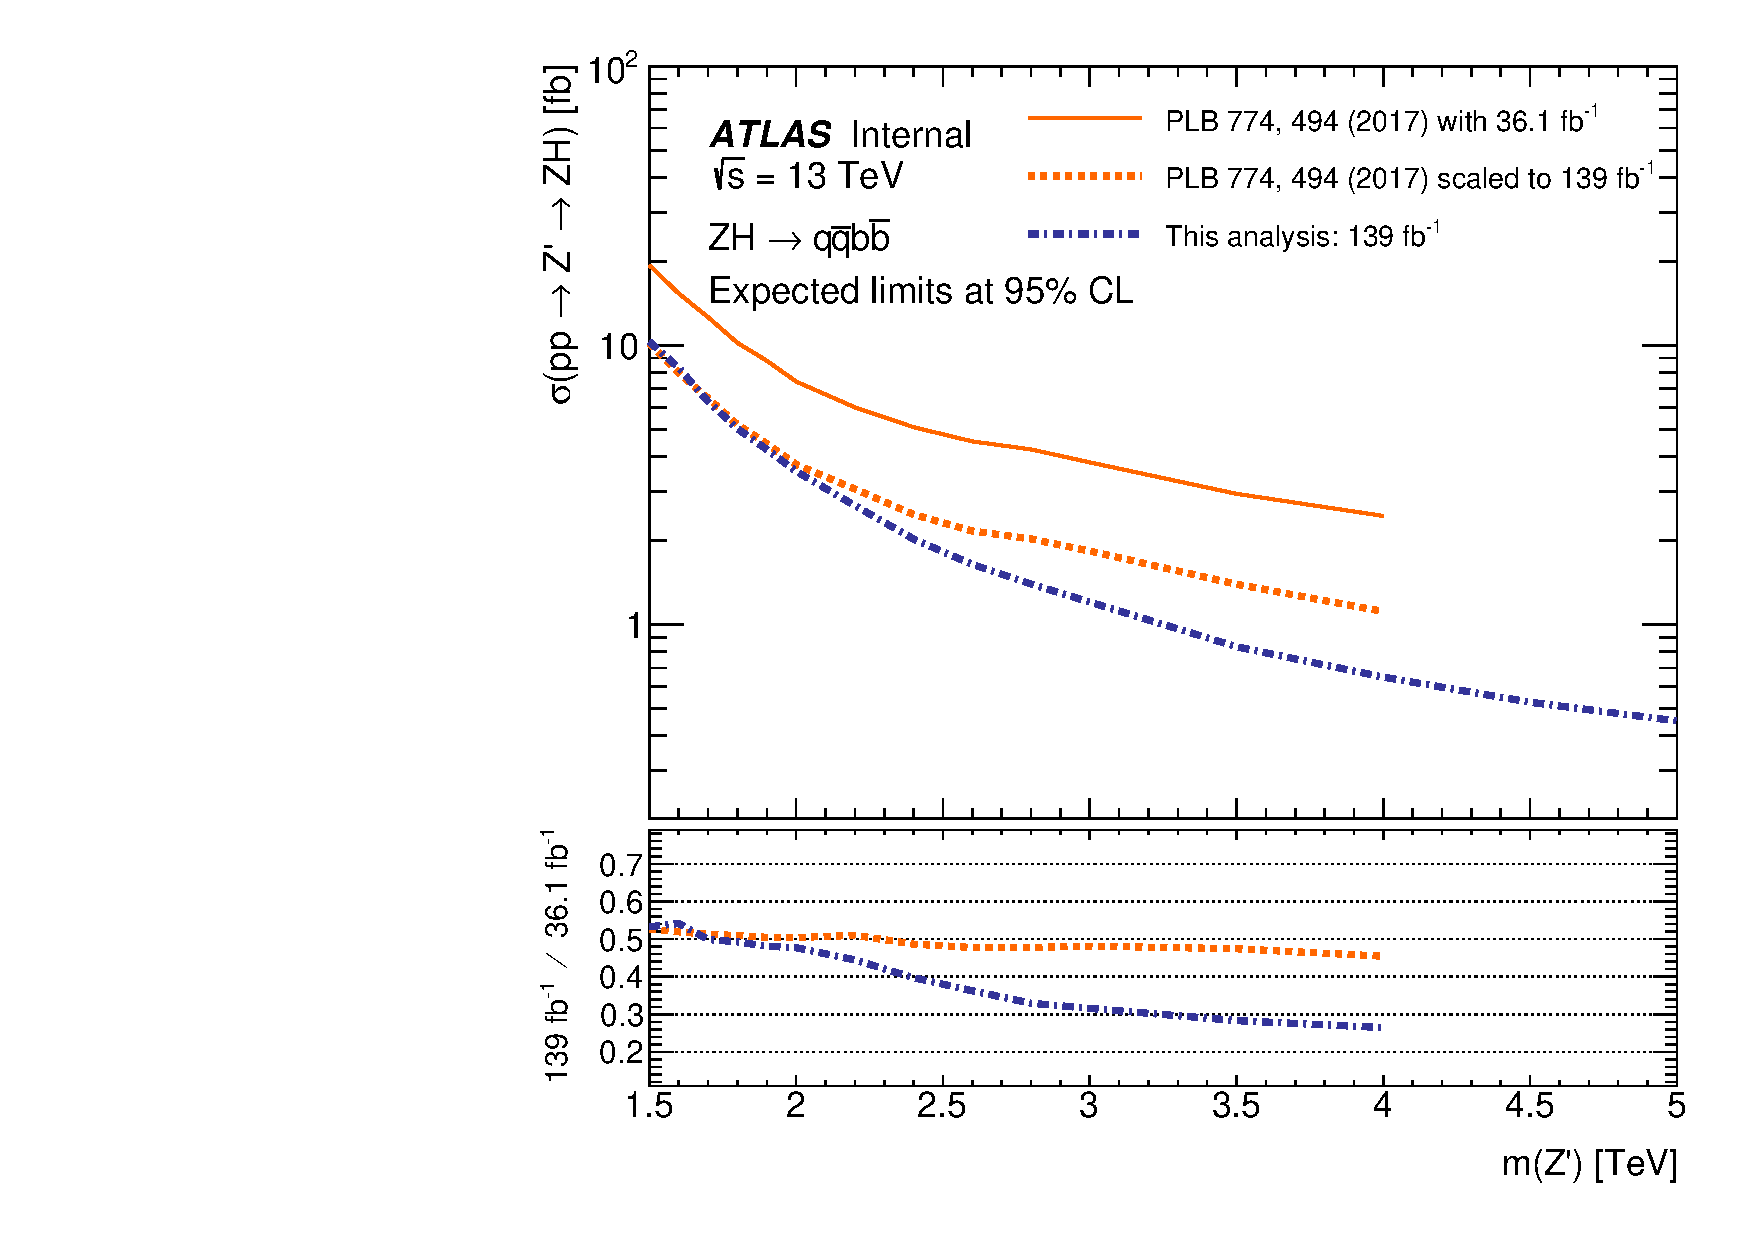
\includegraphics[width=0.65\textwidth]{VHqqbbLimit_ZH_2016_2019_v4.pdf}
    \end{center}
    \caption{
        A comparison of expected limits for the WH (top) and ZH (bottom) final states including the previous result published in Phys. Lett. B 774.
        The solid red line shows the published limit, while the dashed red line shows that same with background and signal scaled to match the full Run-2 luminosity.
        The dashed blue line shows the expected limit results for the current strategy described in this thesis for the full Run-2 luminosity.
    }
    \label{fig:exp_limit_cmp}
\end{figure}

\begin{figure}[htbp!]
    \begin{center}
        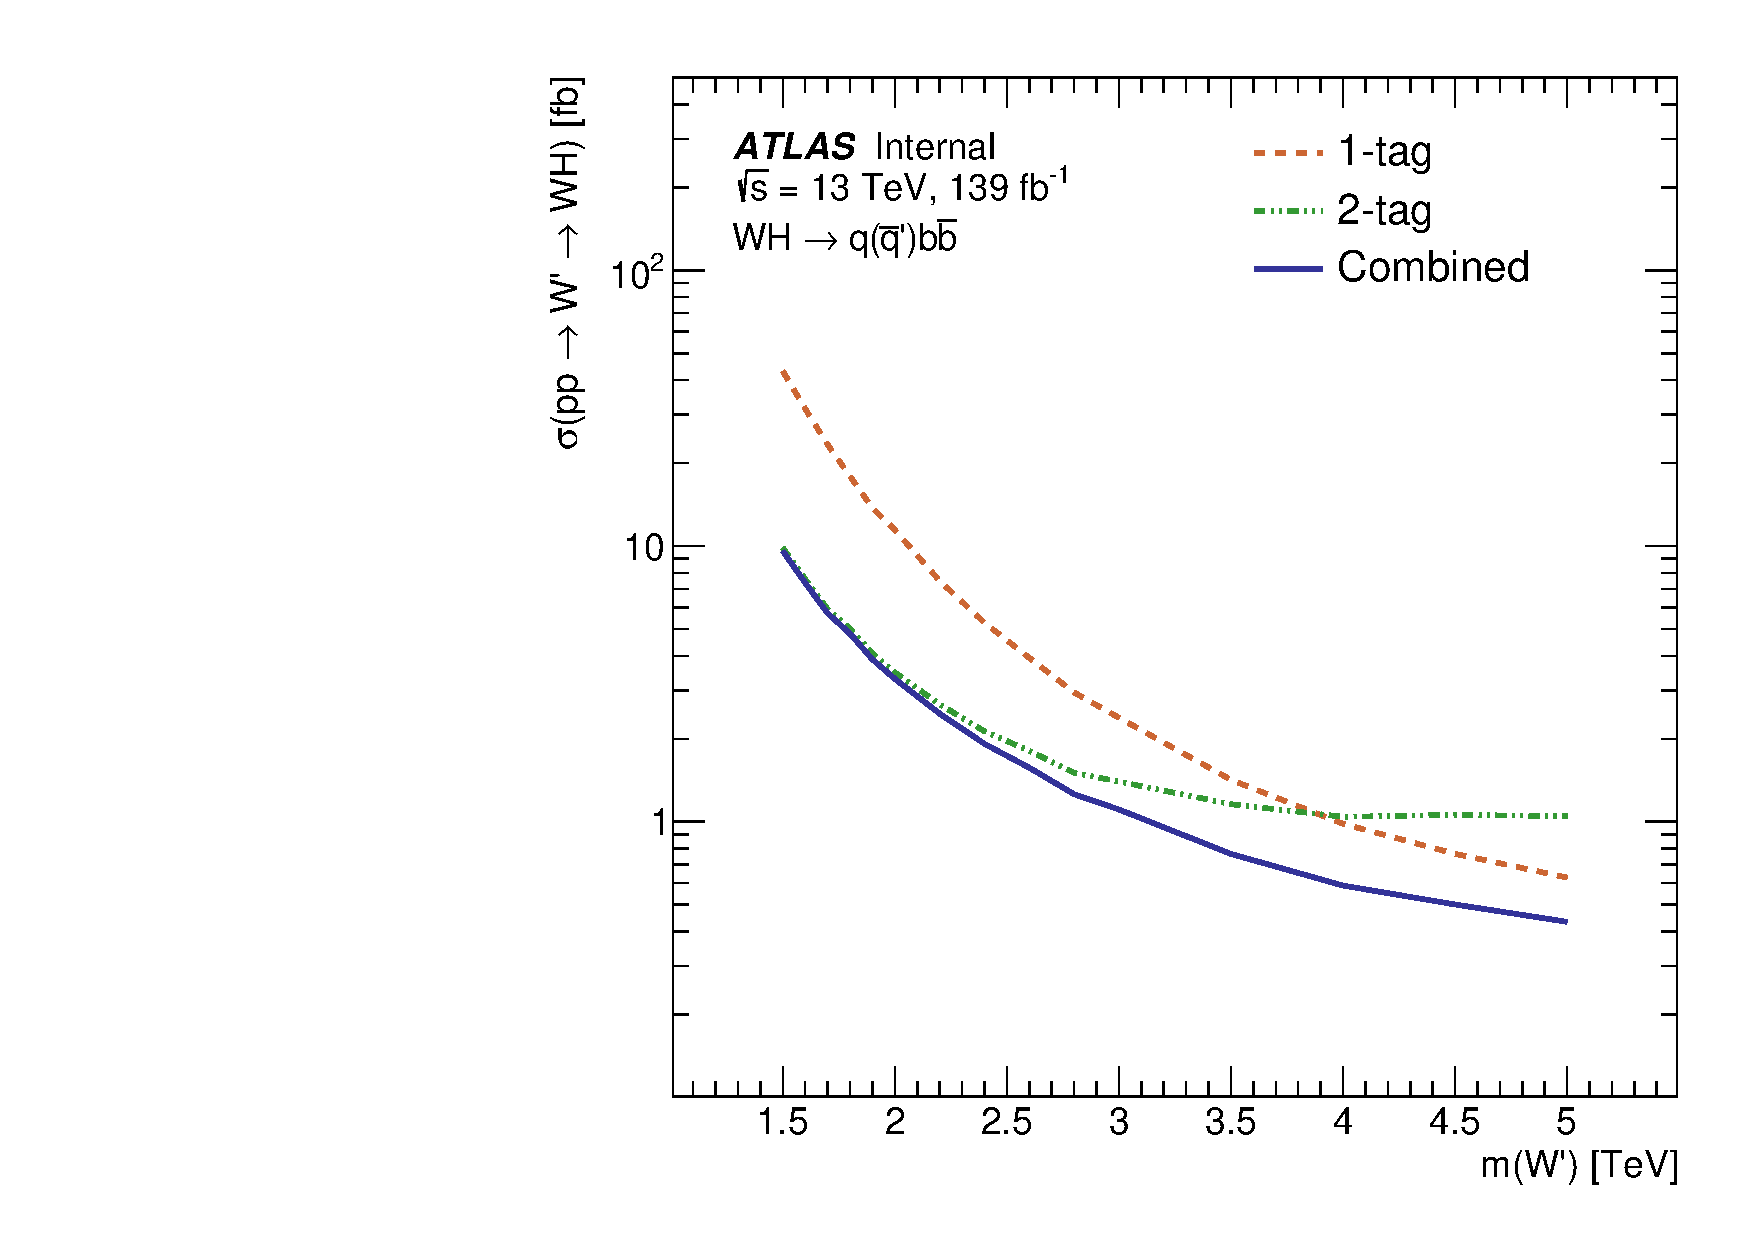
\includegraphics[width=0.49\textwidth]{VHqqbbLimit_WH_channels.pdf}
        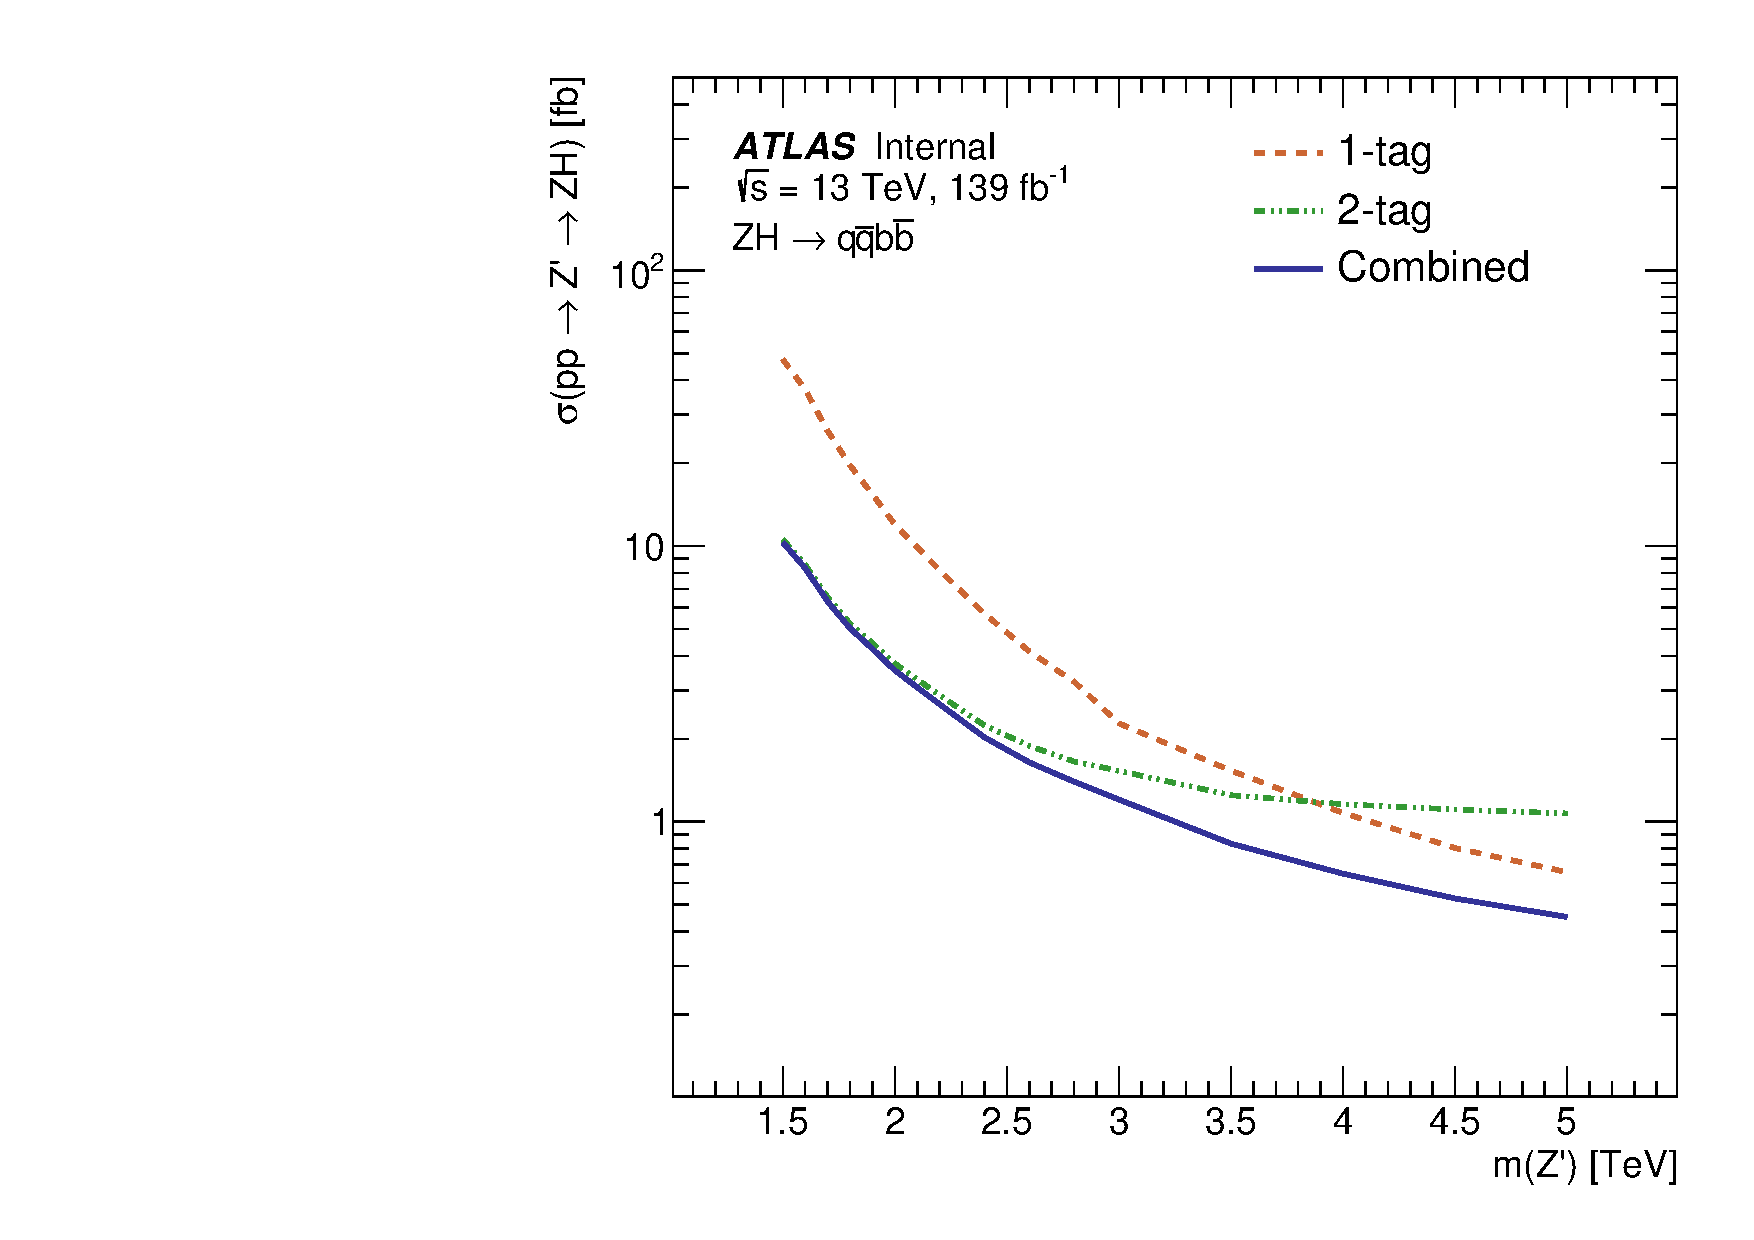
\includegraphics[width=0.49\textwidth]{VHqqbbLimit_ZH_channels.pdf}
    \end{center}
    \caption{Upper limits on $\sigma(V^\prime \rightarrow VH) \times BR(H \rightarrow b\bar{b})$ at 95\% CL for WH (left) and ZH (right) channels.
        The figures show the expected limits for each channel: 1-tag (dashed orange), 2-tag (dashed green), and combined (solid blue).
    }
    \label{fig:exp_limit_channels}
\end{figure}

% \begin{figure}[htbp!]
%     \begin{center}
%         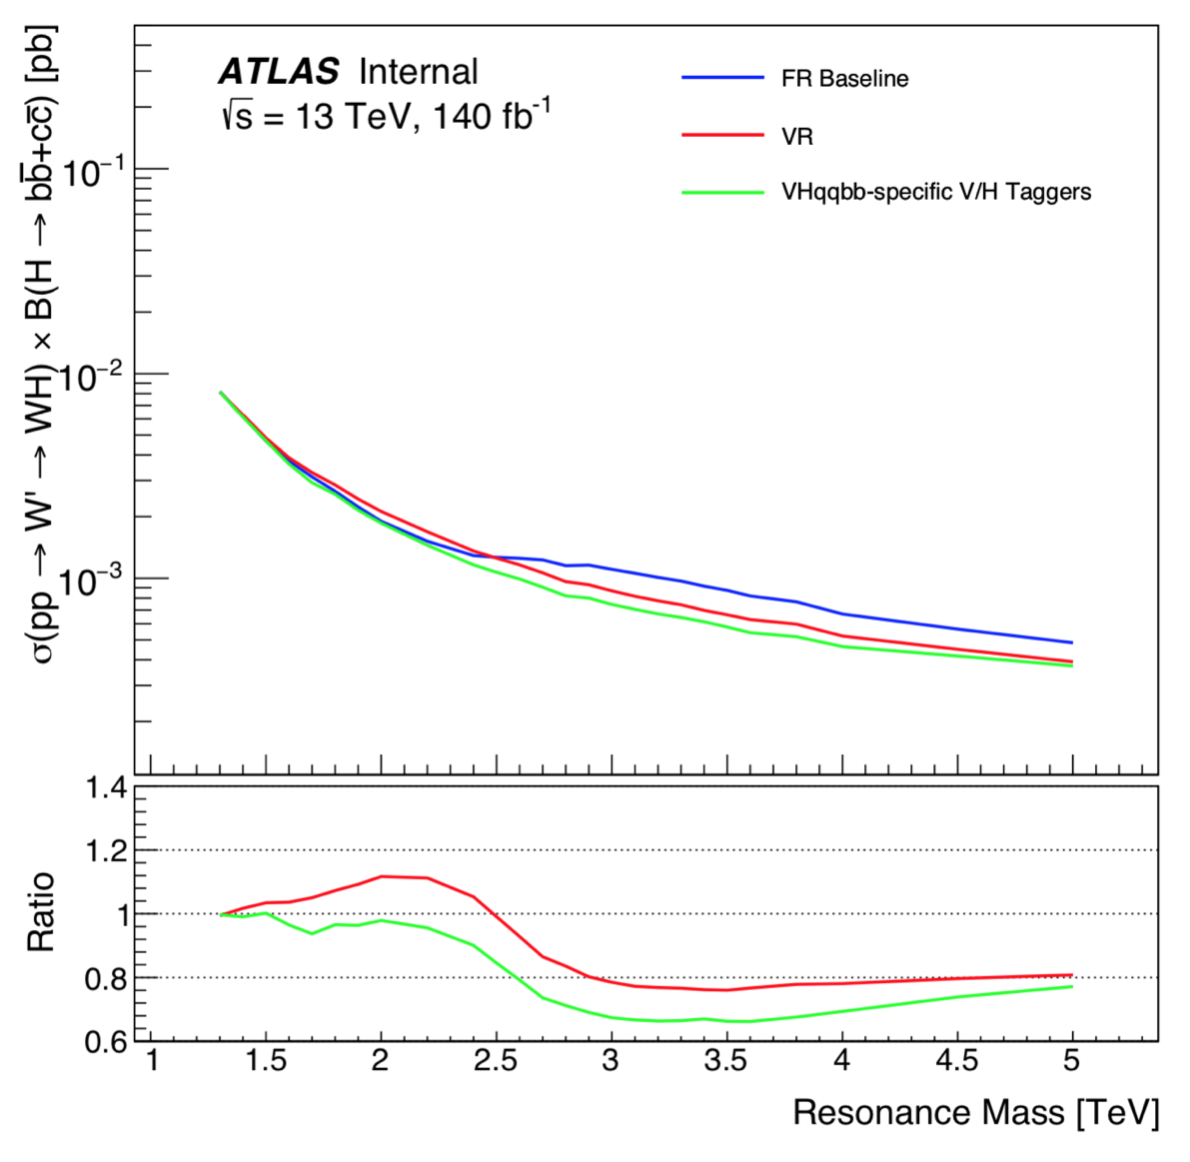
\includegraphics[width=0.65\textwidth]{improvements.png} \\
%     \end{center}
%     \caption{
%         A breakdown of expected limits improvements coming from variable radius track jets (red) and updated H/W/Z taggers (green).
%         The nominal \textit{FR baseline} (blue) was produced using fixed radius track jets, VVJJ W/Z boson taggers, and a fixed Higgs mass window of [75,200] GeV.
%         Note that this plot is out of date and doesn't reflect the final analysis selection, so is only intended to outline relative improvements due to VR track jets and updated boson tagging.
%     }
%     \label{fig:exp_limit_improvements}
% \end{figure}

